\section{Διαφορικός λογισμός}
\subsection{Ορισμός και Κανόνες Παραγώγισης}
\begin{askhsh}{Παράγωγος σε σημείο (δίκλαδη συνάρτηση)}
\bhmata\begin{bhma}
\item Βρίσκουμε το πεδίο ορισμού και εξετάζουμε τη συνέχειας της συνάρτησης στο σημείο αλλαγής τύπου $x_0$. Αν η συνάρτηση δεν είναι συνεχής στο $x_0$, τότε δεν είναι παραγωγίσιμη σε αυτό.
\item Αν είναι συνεχής στο $x_0$, υπολογίζουμε τα πλευρικά όρια του λόγου μεταβολής:
\[ \lim\limits_{x\to x_0^-}\frac{f(x)-f(x_0)}{x-x_0} \quad \text{και} \quad \lim\limits_{x\to x_0^+}\frac{f(x)-f(x_0)}{x-x_0} \]
\item Αν τα δύο πλευρικά όρια υπάρχουν, είναι πραγματικοί αριθμοί και είναι ίσα (έστω $l$), τότε η συνάρτηση είναι παραγωγίσιμη στο $x_0$ με $f'(x_0) = l$.
\end{bhma}
\end{askhsh}

\Paradeigma{Παράγωγος δίκλαδης συνάρτησης σε σημείο}
\bmath{Να εξετάσετε αν η συνάρτηση $f(x) = \begin{cases} x^2+x+1, & x \le 0 \\ \hm x + 1, & x > 0 \end{cases}$ είναι παραγωγίσιμη στο $x_0=0$.}

\lysh
Εξετάζουμε πρώτα τη συνέχεια της $f$ στο $x_0=0$:
\begin{multicols}{2}
\begin{itemize}
\item $f(0) = 0^2+0+1 = 1$
\item $\lim\limits_{x\to 0^-} f(x) = \lim\limits_{x\to 0^-} (x^2+x+1) = 1$
\item $\lim\limits_{x\to 0^+} f(x) = \lim\limits_{x\to 0^+} (\hm x + 1) = 1$
\end{itemize}
\end{multicols}
Αφού $\lim\limits_{x\to 0^-} f(x) = \lim\limits_{x\to 0^+} f(x) = f(0)$, η $f$ είναι συνεχής στο $0$. Ελέγχουμε τώρα την παραγωγισιμότητα υπολογίζοντας τις πλευρικές παραγώγους:
\begin{itemize}
\item Για $x < 0$: 
\[ \lim\limits_{x\to 0^-} \frac{f(x)-f(0)}{x-0} = \lim\limits_{x\to 0^-} \frac{x^2+x+1-1}{x} = \lim\limits_{x\to 0^-} \frac{x^2+x}{x} = \lim\limits_{x\to 0^-} (x+1) = 1 \]
\item Για $x > 0$: 
\[ \lim\limits_{x\to 0^+} \frac{f(x)-f(0)}{x-0} = \lim\limits_{x\to 0^+} \frac{\hm x + 1 - 1}{x} = \lim\limits_{x\to 0^+} \frac{\hm x}{x} = 1 \]
\end{itemize}
Επειδή $\lim\limits_{x\to 0^-} \frac{f(x)-f(0)}{x-0} = \lim\limits_{x\to 0^+} \frac{f(x)-f(0)}{x-0} = 1$, η $f$ είναι παραγωγίσιμη στο $0$ με $f'(0) = 1$.

\begin{askhsh}{Κανόνες παραγώγισης}
\bhmata\begin{bhma}
\item Αναγνωρίζουμε αν πρόκειται για απλή ή σύνθετη συνάρτηση.
\item Εφαρμόζουμε τους βασικούς κανόνες παραγώγισης. (Πίνακας \ref{pinakas:kanones_paragwgisis})
\item Υπολογίζουμε τις παραγώγους των βασικών συναρτήσεων (Πίνακας \ref{pinakas:paragwgoi}) που προκύπτουν και κάνουμε τις απαραίτητες πράξεις.
\end{bhma}
\end{askhsh}
\begin{center}\label{pinakas:paragwgoi}
\begin{mytblr}{rowhead = 2,row{1-2} = {maincolor!70!black,fg={white}},row{2}={font=\bf},cell{1-2}{3-5} = {secondcolor!90!black},cell{even[4-Z]}{3-5} = {secondcolor!70!white},cell{odd[3-Z]}{3-5} = {secondcolor!30!white}}
\SetCell[c=2]{c} ΑΠΛΕΣ & & \SetCell[c=3]{c} ΣΥΝΘΕΤΕΣ & &  \\ 
Συνάρτηση $ f $& Παράγωγος $ f' $ & Συνάρτηση $ g\circ f $ & Παράγωγος $ \left( g\circ f \right)' $ & Λεκτική περιγραφή \\ 
$ c $ & $ 0 $ &  & & \\ 
$ x $ & $ 1 $ &  & & \\ 
$ x^\nu $ & $ \nu x^{\nu-1} $ & $ f^\nu(x) $ & $ \nu f^{\nu-1}(x)\cdot f'(x) $ & $ \nu(\text{βάση})^{\nu-1}(\text{βαση})' $\\ 
$ \dfrac{1}{x} $ & $ -\dfrac{1}{x^2} $ & $ \dfrac{1}{f(x)} $ & $ -\dfrac{f'(x)}{f^2(x)} $ &$ -\dfrac{(\text{Παρονομαστής})'}{\text{Παρονομαστής}^2} $ \\ 
$ \sqrt{x} $ & $ \dfrac{1}{2\!\sqrt{x}} $ & $ \sqrt{f(x)} $ & $ \dfrac{f'(x)}{2\!\sqrt{f(x)}} $ & $ \dfrac{(\text{Υπόριζο})'}{2\cdot\text{Ρίζα}} $ \\ 
$ \hm{x} $ & $ \syn{x} $ & $ \hm{f(x)} $ & $ \syn{f(x)}\cdot f'(x) $ & $ \syn{(\text{Γωνία})\cdot(\text{Γωνία})'} $\\ 
$ \syn{x} $ & $ -\hm{x} $ & $ \syn{f(x)} $ & $ -\hm{f(x)}\cdot f'(x) $ &$ -\hm{(\text{Γωνία})\cdot(\text{Γωνία})'} $ \\ 
$ \ef{x} $ & $ \dfrac{1}{\syn^2{x}} $ & $ \ef{f(x)} $ & $ \dfrac{f'(x)}{\syn^2{f(x)}} $ & $ \dfrac{(\text{Γωνία})'}{\syn^2{(\text{Γωνία})}} $ \\ 
$ \syf{x} $ & $ -\dfrac{1}{\hm^2{x}} $ & $ \syf{f(x)} $ & $ -\dfrac{f'(x)}{\hm^2{f(x)}} $ & $ -\dfrac{(\text{Γωνία})'}{\hm^2{(\text{Γωνία})}} $ \\ 
$ a^x $ & $ a^x\ln{a} $ & $ a^{f(x)} $ & $ a^{f(x)}\ln{a}\cdot f'(x) $ & $ a^{\text{Εκθέτης}}\cdot\ln{a}\cdot(\text{Εκθέτης})' $ \\ 
$ e^x $ & $ e^x $ & $ e^{f(x)} $ & $ e^{f(x)}\cdot f'(x) $ & $ e^{\text{Εκθέτης}}\cdot(\text{Εκθέτης})' $ \\ 
$ \ln{x} $ & $ \dfrac{1}{x} $ & $ \ln{f(x)} $ & $ \dfrac{f'(x)}{f(x)} $ & $ \dfrac{(\text{Παράσταση})'}{\text{Παράσταση}} $
\end{mytblr}\captionof{table}{Παράγωγοι απλών και σύνθετων συναρτήσεων}
\end{center}
\Paradeigma{Παράγωγος απλών συναρτήσεων}
\bmath{Να βρείτε την παράγωγο της συνάρτησης 
\begin{multicols}{2}
\begin{alist}
\item $f(x)=x^2\ln{x}$
\item $f(x) = \dfrac{e^x}{x^2+1}$.
\end{alist}
\end{multicols}
}

\lysh\label{pinakas:kanones_paragwgisis}
\wrapr{-10mm}{10}{7cm}{-5mm}{
\begin{mytblr}{}
Συνάρτηση & Παράγωγος\\
$f(x)\pm g(x)$ & $f'(x)+g'(x)$\\
$c\cdot f(x)$ & $c\cdot f'(x)$\\
$f(x)\cdot g(x)$ & $f'(x)g(x)+f(x)g'(x)$\\
$\dfrac{f(x)}{g(x)}$ & $\dfrac{f'(x)g(x)-f(x)g'(x)}{g^2(x)}$\\
$f(g(x))$ & $f'(g(x))g'(x)$
\end{mytblr}\captionof{table}{Κανόνες παραγώγισης}
}{
\begin{alist}
\item Η $f$ ορίζεται όταν $x>0$ άρα $D_f=(0,+\infty)$. Για κάθε $x>0$ σύμφωνα με τον κανόνα του γινομένου είναι:
\begin{align*}
f'(x)&=\left(x^2\ln{x}\right)'=(x^2)'\ln{x}+x^2\left(\ln{x}\right)'=\\
&=2x\ln{x}+x^2\cdot \frac{1}{x}=2x\ln{x}+x=x(2\ln{x}+1)
\end{align*}
\item 
Η συνάρτηση $f$ ορίζεται στο $D_f=\mathbb{R}$. Σύμφωνα με τον κανόνα του πηλίκου, για κάθε $x\in\mathbb{R}$ έχουμε:
\begin{align*}
f'(x) &= \left(\frac{e^x}{x^2+1}\right)' = \frac{(e^x)'(x^2+1) - e^x(x^2+1)'}{(x^2+1)^2} =\\
&= \frac{e^x(x^2+1) - e^x(2x)}{(x^2+1)^2} = \frac{e^x(x^2 - 2x + 1)}{(x^2+1)^2} = \frac{e^x(x-1)^2}{(x^2+1)^2}
\end{align*}
\end{alist}
}

\Paradeigma{Παράγωγος σύνθετης συνάρτησης}
\bmath{Να βρείτε την παράγωγο της συνάρτησης $f(x) = \ln(x^2+3x+5) + \hm^3(2x)$.}

\lysh
Η συνάρτηση $f$ είναι άθροισμα δύο σύνθετων συναρτήσεων. Εφαρμόζουμε τον κανόνα της αλυσίδας για καθεμία ξεχωριστά:
\begin{align*}
f'(x) &= [\ln(x^2+3x+5)]' + [\hm^3(2x)]' \\
&= \frac{1}{x^2+3x+5} \cdot (x^2+3x+5)' + 3\hm^2(2x) \cdot (\hm(2x))' \\
&= \frac{1}{x^2+3x+5} \cdot (2x+3) + 3\hm^2(2x) \cdot \syn(2x) \cdot (2x)' \\
&= \frac{2x+3}{x^2+3x+5} + 3\hm^2(2x) \syn(2x) \cdot 2 \\
&= \frac{2x+3}{x^2+3x+5} + 6\hm^2(2x) \syn(2x)
\end{align*}

\subsection{Εφαπτομένη}
\begin{askhsh}{Εύρεση εφαπτομένης με γνωστό σημείο επαφής}
\bhmata\begin{bhma}
\item Βρίσκουμε το πεδίο ορισμού και παράγωγο $ f'(x) $.
\item Υπολογίζουμε τις τιμές $ f(x_0) $ και $ f'(x_0) $.
\item Γράφουμε την εξίσωση της ευθείας
\[ y-f(x_0)=f'(x_0)(x-x_0) \]
και αντικαθιστώντας λύνουμε ως προς $ y $.
\end{bhma}
\end{askhsh}
\Paradeigma{Εφαπτομένη - Γνωστό σημείο επαφής}
\bmath{Δίνεται η συνάρτηση $f(x)=\frac{e^x}{x-1}$. Να βρεθεί η εξίσωση της εφαπτόμενης ευθείας της $C_f$ στο σημείο
\begin{multicols}{2}
\begin{alist}
\item $M(0,f(0))$
\item με τετμημένη $-1$.
\end{alist}
\end{multicols}}

\lysh
Η $f$ ορίζεται όταν $x-1\neq 0\Rightarrow x\neq 1$ άρα $D_f=\mathbb{R}-\{1\}$. Για κάθε $x\in\mathbb{R}-\{1\}$:
\[f'(x)=\left(\frac{e^x}{x-1}\right)'=\frac{\left(e^x\right)'(x-1)-e^x(x-1)'}{(x-1)^2}=\frac{e^x(x-1)-e^x}{(x-1)^2}=\frac{e^x(x-2)}{(x-1)^2}\]
\begin{alist}
\item Για $x=0$ έχουμε:
\begin{multicols}{2}
\begin{itemize}
\item $f(0)=\dfrac{e^0}{0-1}=-1$ και 
\item $f'(0)=\dfrac{e^0(0-2)}{(0-1)^2}=-2$
\end{itemize}
\end{multicols}
άρα η εξίσωση της εφαπτομένης στο $M$ θα είναι
\begin{gather*}
y-f(0)=f'(0)(x-0)\Rightarrow\\
y-(-1)=-2x\Rightarrow y=-2x-1
\end{gather*}
\item Για $x=-1$ έχουμε
\begin{multicols}{2}
\begin{itemize}
\item $f(-1)=\dfrac{e^{-1}}{-1-1}=-\dfrac{1}{2e}$
\item $f'(-1)=\dfrac{e^{-1}(-1-2)}{(-1-1)^2}=\dfrac{-3}{4e}$
\end{itemize}
\end{multicols}
επομένως η εφαπτομένη στο σημείο $M\left(-1,-\frac{1}{2e}\right)$ έχει εξίσωση
\begin{gather*}
y-f(-1)=f'(-1)(x+1)\Rightarrow
y-\left(-\frac{1}{2e}\right)=-\frac{3}{4e}(x+1)\Rightarrow\\
y=-\frac{3}{4e}x-\frac{5}{4e}
\end{gather*}
\end{alist}
\begin{askhsh}{Εύρεση εφαπτομένης με γνωστή κλίση λ}
\bhmata\begin{bhma}
\item Βρίσκουμε το πεδίο ορισμού της $f$, την $ f'(x) $ και θεωρούμε σημείο επαφής $ M(x_0,f(x_0)) $.
\item  Βρίσκουμε το συντελεστή διεύθυνσης $ \lambda $ της εφαπτομένης και σχηματίζουμε την εξίσωση
\[ f'(x_0)=\lambda \]
Αν δεν μας δίνεται ο συντελεστής $ \lambda $ της εφαπτομένης $ \varepsilon $ τότε τον βρίσκουμε με τη βοήθεια του παρακάτω πίνακα:
\begin{center}
\begin{mytblr}{cc}
\textbf{Συνθήκη} & \textbf{Εξίσωση} \\
Ευθείες παράλληλες $ \varepsilon\parallel \zeta $ &$ \lambda_{\varepsilon}=\lambda_{\zeta}\Rightarrow f'(x_0)=\lambda $  \\
Ευθείες κάθετες $ \varepsilon\perp\zeta $ & $ \lambda_{\varepsilon}\cdot\lambda_{\zeta}=-1\Rightarrow \ldots\Rightarrow f'(x_0)=\lambda $ \\
Οριζόντια ευθεία $ \varepsilon\parallel x'x $  & $ \lambda_{\varepsilon}=0\Rightarrow f'(x_0)=0 $ \\
Η $ \varepsilon $ σχηματίζει γωνία $ \omega $ & $ \lambda_{\varepsilon}=\ef{\omega}\Rightarrow f'(x_0)=\ef{\omega} $.
\end{mytblr}\captionof{table}{Συντελεστές διεύθυνσης ευθειών}
\end{center}
\item Λύνουμε την εξίσωση, βρίσκουμε το $ x_0 $ και στη συνέχεια το $ f(x_0) $.
\item Γράφουμε την εξίσωση της ευθείας $ y-f(x_0)=f'(x_0)(x-x_0) $.
\end{bhma}
\end{askhsh}
\Paradeigma{Εφαπτομένη με γνωστή κλίση}
\bmath{Δίνεται η συνάρτηση $f:\mathbb{R}\to\mathbb{R}$ με τύπο $f(x)=x^2-3x+1$. Να βρείτε την εξίσωση της εφαπτομένης η οποία
\begin{alist}
\item έχει συντελεστή διεύθυνσης $\lambda=3$.
\item είναι παράλληλη με την ευθεία $\zeta:y=-5x+2$.
\item είναι κάθετη στην ευθεία $\eta:y=\frac{1}{3}x-1$.
\item είναι παράλληλη με τον άξονα $x'x$.
\item σχηματίζει γωνία $135\degree$ με τον άξονα $x'x$.
\end{alist}}

\lysh
Έστω $M(x_0,f(x_0))$ το σημείο επαφής. Για κάθε $x\in\mathbb{R}$ είναι
\[f'(x)=\left(x^2-3x+1\right)'=2x-3\]
\begin{alist}
\item Η εφαπτομένη $\varepsilon$ έχει κλίση $\lambda=3$ άρα
\[f'(x_0)=3\Rightarrow2x_0-3=3\Rightarrow2x_0=6\Rightarrow x_0=3\]
άρα η τεταγμένη του σημείου επαφής είναι $f(3)=3^2-3\cdot3+1=1$. Έτσι η εξίσωση της $\varepsilon$ θα είναι
\begin{gather*}
y-f(3)=f'(3)(x-3)\Rightarrow\\
y-1=3(x-3)\Rightarrow y=3x-8
\end{gather*}
\item Η $\varepsilon$ είναι παράλληλη με την $\zeta$ οπότε ισχύει
\[\varepsilon\parallel\zeta\Rightarrow\lambda_{\varepsilon}=\lambda_{\zeta}\Rightarrow f'(x_0)=-5\Rightarrow 2x_0-3=-5\Rightarrow 2x_0=-2\Rightarrow x_0=-1\]
έτσι η τεταγμένη του σημείου επαφής είναι $f(-1)=(-1)^2-3\cdot(-1)+1=1+3+1=5$. Η $\varepsilon$ έχει εξίσωση 
\begin{gather*}
y-f(-1)=f'(-1)(x+1)\Rightarrow
y-5=-5(x+1)\Rightarrow y=-5x
\end{gather*}
\item Η $\varepsilon$ είναι κάθετη στην ευθεία $\eta$ άρα ισχύει
\begin{gather*}
\varepsilon\perp\eta\Rightarrow \lambda_{\varepsilon}\cdot\lambda_{\eta}=-1\Rightarrow f'(x_0)\cdot\frac{1}{3}=-1\Rightarrow f'(x_0)=-3\Rightarrow\\
2x_0-3=-3\Rightarrow 2x_0=0\Rightarrow x_0=0
\end{gather*}
Το σημείο επαφής έχει τεταγμένη $f(0)=0^2-3\cdot 0+1=1$ και η εφαπτομένη έχει εξίσωση
\[y-f(0)=f'(0)(x-0)\Rightarrow y-1=-3x\Rightarrow y=-3x+1\]
\item Η $\varepsilon$ είναι παράλληλη στον άξονα $x'x$ άρα
\[\lambda_{\varepsilon}=0\Rightarrow f'(x_0)=0\Rightarrow 2x_0-3=0\Rightarrow 2x_0=3\Rightarrow x_0=\frac{3}{2}\]
Το σημείο $M$ έχει τεταγμένη
\[ f\left(\frac{3}{2}\right)=\left(\frac{3}{2}\right)^2-3\cdot\frac{3}{2}+1=\frac{9}{4}-\frac{9}{2}+1=-\frac{5}{4} \]
άρα η εφαπτομένη θα έχει εξίσωση
\[ y-f\left(\frac{3}{2}\right)=f'\left(\frac{3}{2}\right)\left(x-\frac{3}{2}\right)\Rightarrow y-\left(-\frac{5}{4}\right)=0\Rightarrow y=-\frac{5}{4} \]
\item Η $\varepsilon$ σχηματίζει γωνία $135\degree$ με τον οριζόντιο άξονα επομένως
\[ \lambda_{\varepsilon}=\ef{135\degree}\Rightarrow f'(x_0)=-1\Rightarrow 2x_0-3=-1\Rightarrow 2x_0=2\Rightarrow x_0=1 \]
Η τεταγμένη του $M$ θα είναι $f(1)=1^2-3\cdot 1+1=-1$ άρα η $\varepsilon$ έχει εξίσωση
\[ y-f(1)=f'(1)(x-1)\Rightarrow y-(-1)=-(x-1)\Rightarrow y=-x \]
\end{alist}
\begin{askhsh}{Εφαπτομένη που διέρχεται από εξωτερικό σημείο $ P(a,\beta) $}
\bhmata\begin{bhma}
\item Πεδίο ορισμού και $ f' $.
\item Θεωρούμε σημείο επαφής $ M(x_0,f(x_0)) $ και γράφουμε τον τύπο της ευθείας.
\item Αντικαθιστούμε $ f(x_0) $ και $ f'(x_0) $ στην εξίσωση.
\item Αφού $ P\in\varepsilon $ τότε θέτουμε $ x=a $ και $ y=\beta $ και λύνουμε την εξίσωση ως προς $ x_0 $.
\item Για κάθε $ x_0 $ υπολογίζουμε $ f(x_0) $ και $ f'(x_0) $ και βρίσκουμε την ευθεία.
\end{bhma}
\end{askhsh}
\Paradeigma{Εύρεση εφαπτομένων που διέρχονται από το $P(a,\beta)$}
\bmath{Δίνεται η συνάρτηση $f(x) = x^2 - 4x + 3$. Να βρείτε τις εξισώσεις των εφαπτομένων της $C_f$ που διέρχονται από το σημείο $P(2, -5)$.}

\lysh
Η συνάρτηση είναι πολυωνυμική, άρα ορίζεται στο $D_f = \mathbb{R}$. Η παράγωγος είναι:
\[ f'(x) = (x^2 - 4x + 3)' = 2x - 4 \]
Έστω $M(x_0, f(x_0))$ το σημείο επαφής. Η εξίσωση της εφαπτομένης $(\varepsilon)$ στο $M$ είναι:
\[ y - f(x_0) = f'(x_0)(x - x_0) \]
Αντικαθιστούμε τα $f(x_0)$ και $f'(x_0)$:
\[ y - (x_0^2 - 4x_0 + 3) = (2x_0 - 4)(x - x_0) \quad \text{(1)} \]
Αφού η εφαπτομένη διέρχεται από το $P(2, -5)$, οι συντεταγμένες του επαληθεύουν την (1). Θέτουμε όπου $x = 2$ και $y = -5$:

\begin{align*}
-5 - (x_0^2 - 4x_0 + 3) &= (2x_0 - 4)(2 - x_0)\\
-5 - x_0^2 + 4x_0 - 3 &= 4x_0 - 2x_0^2 - 8 + 4x_0 \\
-x_0^2 + 4x_0 - 8 &= -2x_0^2 + 8x_0 - 8 \\
2x_0^2 - x_0^2 + 4x_0 - 8x_0 - 8 + 8 &= 0 \\
x_0^2 - 4x_0 &= 0 \\
x_0(x_0 - 4) &= 0
\end{align*}
Άρα προκύπτουν δύο λύσεις (δύο σημεία επαφής):
\[ x_0 = 0 \quad \text{ή} \quad x_0 = 4 \]
\begin{itemize}
    \item \textbf{Για $\mathbf{x_0 = 0}$:}
    \\
    Βρίσκουμε την κλίση και το σημείο επαφής:
    \[ f'(0) = 2(0) - 4 = -4 \]
    \[ f(0) = 0^2 - 4(0) + 3 = 3 \]
    Η εξίσωση της εφαπτομένης ($\varepsilon_1$) είναι:
    \[ y - 3 = -4(x - 0) \Rightarrow {y = -4x + 3} \]

    \item \textbf{Για $\mathbf{x_0 = 4}$:}
    \\
\wrapr{-5mm}{10}{6.2cm}{-15mm}{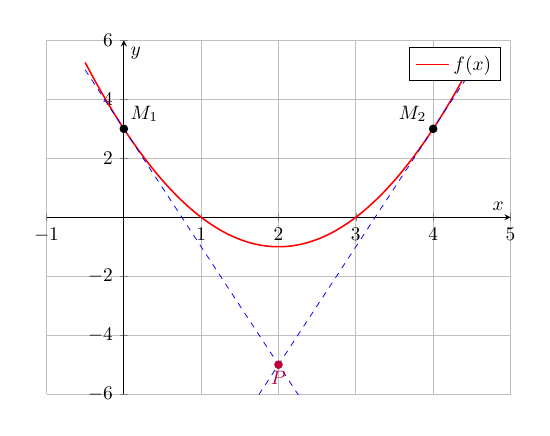
\begin{tikzpicture}[scale=0.7]
    \begin{axis}[
        axis lines = middle,
        xlabel = $x$,
        ylabel = $y$,
        xmin = -1, xmax = 5,
        ymin = -6, ymax = 6,
        grid = both,
        width=10cm, height=8cm
    ]
    % Function f(x) = x^2 - 4x + 3
    \addplot [domain=-0.5:4.5, samples=100, color=red, thick] {x^2 - 4*x + 3};
    \addlegendentry{$f(x)$}
    
    % Tangent 1: y = -4x + 3
    \addplot [domain=-0.5:2.5, samples=2, color=blue, dashed] {-4*x + 3};
    
    % Tangent 2: y = 4x - 13
    \addplot [domain=1.5:4.5, samples=2, color=blue, dashed] {4*x - 13};
    
    % Point P
    \addplot[mark=*,purple] coordinates {(2,-5)} node[below] {$P$};
    
    % Contact points
    \addplot[mark=*,black] coordinates {(0,3)} node[above right] {$M_1$};
    \addplot[mark=*,black] coordinates {(4,3)} node[above left] {$M_2$};
    
    \end{axis}
\end{tikzpicture}
}{
    Βρίσκουμε την κλίση και το σημείο επαφής:
    \[ f'(4) = 2(4) - 4 = 8 - 4 = 4 \]
    \[ f(4) = 4^2 - 4(4) + 3 = 16 - 16 + 3 = 3 \]
    Η εξίσωση της εφαπτομένης ($\varepsilon_2$) είναι:
    \[ y - 3 = 4(x - 4) \Rightarrow y - 3 = 4x - 16 \Rightarrow {y = 4x - 13} \]}
\end{itemize}
\begin{askhsh}{Ευθεία εφάπτεται στη $ C_f $ στο $ M(x_0,f(x_0)) $}
\[ \textrm{Η ευθεία }y=ax+\beta\textrm{ εφάπτεται στη }C_f\Leftrightarrow \ccases{f(x_0)=ax_0+\beta\\f'(x_0)=a} \]
\end{askhsh}
\Paradeigma{Ευθεία που εφάπτεται σε γνωστό σημείο}
\bmath{Δίνεται η συνάρτηση $f(x) = \ln x + ax + \beta,\ x>0$. Να βρείτε τις τιμές των $a,\beta \in \mathbb{R}$ ώστε η ευθεία $\varepsilon: y = 2x - 1$ να εφάπτεται στη $C_f$ στο σημείο της $M(1, f(1))$.}

\lysh
Για να εφάπτεται η $(\varepsilon)$ στη $C_f$ στο $M(1, f(1))$, πρέπει το σημείο $M$ να ανήκει στην $(\varepsilon)$ και η παράγωγος της $f$ στο $x_0=1$ να ισούται με την κλίση της $(\varepsilon)$. Δηλαδή:
\[ \ccases{f(1)=2\cdot 1-1\\f'(1)=2} \Rightarrow \ccases{f(1)=1\\f'(1)=2} \]
Η $f$ είναι παραγωγίσιμη στο $(0, +\infty)$ με $f'(x) = \dfrac{1}{x} + a$.
\begin{itemize}
\item Από την $f'(1) = 2$ έχουμε: $\dfrac{1}{1} + a = 2 \Rightarrow a = 1$.
\item Από την $f(1) = 1$ έχουμε: $\ln 1 + a\cdot 1 + \beta = 1 \Rightarrow 0 + 1 + \beta = 1 \Rightarrow \beta = 0$.
\end{itemize}
Άρα $a=1$ και $\beta=0$.
\begin{askhsh}{Κοινή εφαπτομένη $ C_f,C_g $ σε κοινό σημείο $ M(x_0,f(x_0)) $}
\[ \textrm{Οι }C_f\textrm{ και }C_g\textrm{ έχουν κοινή εφαπτομένη στο }Μ\Leftrightarrow \ccases{f(x_0)=g(x_0)\\f'(x_0)=g'(x_0)} \]
\end{askhsh}
\Paradeigma{Κοινή εφαπτομένη σε κοινό σημείο}
\bmath{Δίνονται οι συναρτήσεις $f(x) = x^2 - x + 1$ και $g(x) = -x^2 + 3x - 1$. Να αποδείξετε ότι οι γραφικές τους παραστάσεις έχουν κοινή εφαπτομένη στο σημείο με τετμημένη $x_0=1$.}

\lysh
Για να έχουν κοινή εφαπτομένη στο $x_0=1$, αρκεί να έχουν κοινό σημείο επαφής (δηλαδή $f(1)=g(1)$) και κοινή κλίση στο σημείο αυτό (δηλαδή $f'(1)=g'(1)$).
Υπολογίζουμε τις τιμές των συναρτήσεων:
\begin{itemize}
\item $f(1) = 1^2 - 1 + 1 = 1$.
\item $g(1) = -1^2 + 3\cdot 1 - 1 = 1$.
\end{itemize}
Άρα $f(1) = g(1) = 1$, δηλαδή έχουν κοινό σημείο το $M(1, 1)$.
Υπολογίζουμε τις παραγώγους και τις τιμές τους στο $x_0=1$:
\begin{itemize}
\item $f'(x) = 2x - 1 \Rightarrow f'(1) = 2(1) - 1 = 1$.
\item $g'(x) = -2x + 3 \Rightarrow g'(1) = -2(1) + 3 = 1$.
\end{itemize}
Άρα $f'(1) = g'(1) = 1$.
Αφού $f(1)=g(1)$ και $f'(1)=g'(1)$, οι $C_f$ και $C_g$ διαθέτουν κοινή εφαπτομένη στο σημείο $M(1, 1)$.

\subsection{Ρυθμός Μεταβολής}
\begin{askhsh}{Προβλήματα ρυθμού μεταβολής}
Στα προβλήματα ρυθμού μεταβολής, όλα τα μεγέθη που μεταβάλλονται θεωρούνται συναρτήσεις του χρόνου $t$. Για την επίλυσή τους ακολουθούμε τα εξής βήματα:

\bhmata
\begin{bhma}
\item Εντοπίζουμε από την εκφώνηση τα μεγέθη που μεταβάλλονται (π.χ. συντεταγμένες $x(t), y(t)$, γωνία $\theta(t)$, εμβαδόν $E(t)$ κλπ).
\item Συμβολίζουμε τους γνωστούς αριθμούς είτε ως τιμές των συναρτήσεων είτε ως παραγώγους (ρυθμό μεταβολής).
\item Βρίσκουμε μια \textbf{σχέση} που συνδέει το ζητούμενο μέγεθος με τα δεδομένα μεγέθη, η οποία να ισχύει για \textbf{κάθε} χρονική στιγμή $t$. Συνήθως προκύπτει από γεωμετρικούς ή τριγωνομετρικούς τύπους.
\item \textbf{Παραγωγίζουμε} και τα δύο μέλη της σχέσης ως προς τον χρόνο $t$, χρησιμοποιώντας τον κανόνα της αλυσίδας (αφού τα μεγέθη είναι σύνθετες συναρτήσεις του $t$).
\item \textbf{Αντικαθιστούμε} τις γνωστές τιμές των μεγεθών για τη συγκεκριμένη χρονική στιγμή $t_0$ και λύνουμε ως προς τον ζητούμενο ρυθμό. Αν κάποιο μέγεθος λείπει, το υπολογίζουμε θέτοντας $t=t_0$ στην αρχική σχέση.
\end{bhma}
\end{askhsh}

\Paradeigma{Κινητό σημείο σε γραφική παράσταση}
\bmath{Ένα σημείο $M(x, y)$ κινείται κατά μήκος της καμπύλης $f(x) = x^2$, με $x > 0$. Η τετμημένη $x$ του σημείου απομακρύνεται από την αρχή των αξόνων με σταθερό ρυθμό $2$ μονάδες/sec. Τη χρονική στιγμή $t_0$ που το σημείο διέρχεται από τη θέση με τετμημένη $x(t_0) = 1$, να βρείτε:
\begin{alist}
\item Το ρυθμό μεταβολής της τεταγμένης του σημείου $M$.
\item Το ρυθμό μεταβολής της γωνίας $\theta$ που σχηματίζει η εφαπτομένη της $C_f$ στο σημείο $M$ με τον άξονα $x'x$.
\item Το ρυθμό μεταβολής του εμβαδού του τριγώνου που σχηματίζει η παραπάνω εφαπτομένη με τους άξονες συντεταγμένων.
\end{alist}}

\lysh
Όλα τα μεγέθη είναι συναρτήσεις του χρόνου $t$. Δίνεται ότι $x'(t) = 2$ για κάθε $t>0$, και ψάχνουμε ρυθμούς μεταβολής τη στιγμή $t_0$ όπου $x(t_0) = 1$.
\begin{alist}
\item Η τεταγμένη του $M$ είναι $y(t) = f(x(t)) = [x(t)]^2$. Παραγωγίζοντας και τα δύο μέλη ως προς $t$ παίρνουμε: 
\[ y'(t) = 2x(t) \cdot x'(t) \]
Τη χρονική στιγμή $t_0$, αντικαθιστούμε τα δεδομένα ($x(t_0)=1, x'(t_0)=2$):
\[ y'(t_0) = 2 \cdot x(t_0) \cdot x'(t_0) = 2 \cdot 1 \cdot 2 = 4 \si{ \mu/sec} \]
Άρα η τεταγμένη αυξάνεται με ρυθμό $4$ \si{\mu/sec}.

\item Ο συντελεστής διεύθυνσης της εφαπτομένης της $C_f$ στο $M$ ισούται με την εφαπτομένη της γωνίας $\theta$. Δηλαδή $\ef{\theta(t)} = f'(x(t))$.
Αφού $f'(x) = 2x$, έχουμε για κάθε χρονική στιγμή $t$:
\[ \ef{\theta(t)} = 2x(t) \]
Παραγωγίζουμε και τα δύο μέλη ως προς $t$:
\[ \frac{1}{\sigma\upsilon\nu^2\theta(t)} \cdot \theta'(t) = 2x'(t) \]
Γνωρίζουμε από τη βασική Τριγωνομετρία ότι $\frac{1}{\sigma\upsilon\nu^2\theta} = 1 + \ef^2\theta$. Επομένως:
\[ (1 + \ef^2\theta(t)) \cdot \theta'(t) = 2x'(t) \Rightarrow (1 + [2x(t)]^2) \cdot \theta'(t) = 2x'(t) \Rightarrow (1 + 4x^2(t)) \cdot \theta'(t) = 2x'(t) \]
Τη χρονική στιγμή $t_0$, έχουμε $x(t_0) = 1$ και $x'(t_0) = 2$:
\[ (1 + 4 \cdot 1^2) \cdot \theta'(t_0) = 2 \cdot 2 \Rightarrow 5\theta'(t_0) = 4 \Rightarrow \theta'(t_0) = \frac{4}{5} \si{ rad/sec} \]
Άρα η γωνία αυξάνεται με ρυθμό $0.8$ \si{rad/sec}.

\item Βρίσκουμε την εξίσωση της εφαπτομένης στο σημείο $M(x(t), y(t))$:
\begin{gather*}
y - f(x(t)) = f'(x(t)) \cdot (x - x(t)) \Rightarrow \\
y - x^2(t) = 2x(t) \cdot (x - x(t)) \Rightarrow \\
y = 2x(t)x - 2x^2(t) + x^2(t) \Rightarrow \\
y = 2x(t)x - x^2(t)
\end{gather*}
Βρίσκουμε τα σημεία τομής της εφαπτομένης με τους άξονες:
\begin{itemize}
\item Για $y=0$: $2x(t)x = x^2(t) \Rightarrow x = \frac{x(t)}{2}$ (αφού $x(t)>0$). Άρα τέμνει τον $x'x$ στο $A\left(\frac{x(t)}{2}, 0\right)$.
\item Για $x=0$: $y = -x^2(t)$. Άρα τέμνει τον $y'y$ στο $B(0, -x^2(t))$.
\end{itemize}
Το εμβαδόν $E(t)$ του τριγώνου $OAB$ (όπου $O$ η αρχή των αξόνων) είναι:
\[ E(t) = \frac{1}{2} (OA)(OB) = \frac{1}{2} \left| \frac{x(t)}{2} \right| \cdot |-x^2(t)| = \frac{1}{2} \cdot \frac{x(t)}{2} \cdot x^2(t) = \frac{1}{4}x^3(t) \]
Παραγωγίζουμε τη συνάρτηση του εμβαδού ως προς $t$:
\[ E'(t) = \frac{1}{4} \cdot 3x^2(t) \cdot x'(t) = \frac{3}{4} x^2(t) x'(t) \]
Τη χρονική στιγμή $t_0$, το εμβαδόν μεταβάλλεται με ρυθμό:
\[ E'(t_0) = \frac{3}{4} x^2(t_0) x'(t_0) = \frac{3}{4} \cdot 1^2 \cdot 2 = \frac{6}{4} = \frac{3}{2} \si{ \tau\mu/sec} \]
Άρα το εμβαδόν αυξάνεται με ρυθμό $1.5$ τετραγωνικές μονάδες ανά δευτερόλεπτο.
\end{alist}

\subsection{Θεώρημα \en{Rolle}}
\begin{askhsh}{Εφαρμογή Θεωρήματος \en{Rolle}}
Για να εφαρμόσουμε το Θεώρημα \en{Rolle} για μια συνάρτηση $f$ σε ένα διάστημα $[\alpha,\beta]$, ελέγχουμε τις εξής τρεις προϋποθέσεις:

\bhmata
\begin{bhma}
\item Η $f$ είναι συνεχής στο κλειστό διάστημα $[\alpha,\beta]$.
\item Η $f$ είναι παραγωγίσιμη στο ανοιχτό διάστημα $(\alpha,\beta)$.
\item Ισχύει $f(\alpha)=f(\beta)$.
\end{bhma}
Αν ισχύουν τα παραπάνω, τότε σύμφωνα με το Θεώρημα \en{Rolle} υπάρχει τουλάχιστον ένα $x_0 \in (\alpha,\beta)$ τέτοιο ώστε $f'(x_0)=0$.
\end{askhsh}
\Paradeigma{Εφαρμογή Θεωρήματος \en{Rolle}}
\bmath{Δίνεται η συνάρτηση $f(x)=x^3-3x^2+2$. Να εξετάσετε αν εφαρμόζεται το Θεώρημα \en{Rolle} για την $f$ στο διάστημα $[0,3]$. Σε περίπτωση που εφαρμόζεται, να βρείτε τα κατάλληλα $x_0 \in (0,3)$ ώστε $f'(x_0)=0$.}

\lysh
Ελέγχουμε τις προϋποθέσεις του Θεωρήματος \en{Rolle} για τη συνάρτηση $f$ στο διάστημα $[0,3]$:
\begin{itemize}
\item Η $f$ είναι συνεχής στο κλειστό διάστημα $[0,3]$ ως πολυωνυμική.
\item Η $f$ είναι παραγωγίσιμη στο ανοιχτό διάστημα $(0,3)$ ως πολυωνυμική, με $f'(x)=3x^2-6x$.
\item Υπολογίζουμε τις τιμές στα άκρα του διαστήματος:
\[ f(0) = 0^3-3\cdot 0^2+2 = 2 \]
\[ f(3) = 3^3-3\cdot 3^2+2 = 27-27+2 = 2 \]
Επομένως ισχύει $f(0)=f(3)$.
\end{itemize}
Αφού ικανοποιούνται όλες οι προϋποθέσεις, το Θεώρημα \en{Rolle} εφαρμόζεται.
Άρα, υπάρχει τουλάχιστον ένα $x_0 \in (0,3)$ τέτοιο ώστε $f'(x_0)=0$. 
Για να βρούμε τα $x_0$, λύνουμε την εξίσωση:
\[ f'(x_0)=0 \Leftrightarrow 3x_0^2-6x_0=0 \Leftrightarrow 3x_0(x_0-2)=0 \]
Από την εξίσωση προκύπτει $x_0=0$ ή $x_0=2$. 
Το $x_0=0$ απορρίπτεται καθώς δεν ανήκει στο ανοιχτό διάστημα $(0,3)$, ενώ το $x_0=2 \in (0,3)$ είναι δεκτό.

\subsection{Θεώρημα Μέσης Τιμής (Θ.Μ.Τ.)}
\begin{askhsh}{Εφαρμογή Θεωρήματος Μέσης Τιμής}
Για να εφαρμόσουμε το Θεώρημα Μέσης Τιμής (Θ.Μ.Τ.) σε μια συνάρτηση $f$ σε ένα διάστημα $[\alpha,\beta]$, ελέγχουμε τις εξής δύο προϋποθέσεις:

\bhmata
\begin{bhma}
\item Η $f$ είναι \textbf{συνεχής} στο κλειστό διάστημα $[\alpha,\beta]$.
\item Η $f$ είναι \textbf{παραγωγίσιμη} στο ανοιχτό διάστημα $(\alpha,\beta)$.
\end{bhma}
Αν ικανοποιούνται οι προϋποθέσεις αυτές, τότε το Θ.Μ.Τ. μας εξασφαλίζει ότι υπάρχει τουλάχιστον ένα $x_0 \in (\alpha,\beta)$ τέτοιο ώστε:
\[ f'(x_0) = \frac{f(\beta)-f(\alpha)}{\beta-\alpha} \]
\textbf{Γεωμετρική Ερμηνεία:} Το κλάσμα $\frac{f(\beta)-f(\alpha)}{\beta-\alpha}$ είναι ο συντελεστής διεύθυνσης $\lambda_{AB}$ της ευθείας (τέμνουσας) που ενώνει τα άκρα $A(\alpha, f(\alpha))$ και $B(\beta, f(\beta))$. Το $f'(x_0)$ είναι η κλίση της εφαπτομένης. Άρα, το θεώρημα μας λέει ότι \textbf{υπάρχει τουλάχιστον ένα σημείο της καμπύλης όπου η εφαπτομένη είναι παράλληλη με την τέμνουσα $AB$}.
\end{askhsh}

\Paradeigma{Θ.Μ.Τ. - Εύρεση σημείου $x_0$ και γεωμετρική ερμηνεία}
\bmath{Δίνεται η συνάρτηση $f(x) = \dfrac{x+2}{x-1}$.
\begin{alist}
\item Να εξετάσετε αν εφαρμόζεται το Θεώρημα Μέσης Τιμής για την $f$ στο διάστημα $[2,4]$.
\item Να βρείτε το σημείο $x_0 \in (2,4)$ στο οποίο η εφαπτομένη της $C_f$ είναι παράλληλη στην ευθεία που ενώνει τα άκρα $A(2,f(2))$ και $B(4,f(4))$.
\end{alist}}

\lysh
\vspace{-5mm}
\begin{alist}
\item Η συνάρτηση ορίζεται όταν $x-1 \neq 0 \Rightarrow x \neq 1$. Άρα το πεδίο ορισμού της είναι το $\mathbb{R}-\{1\}$. 
Παρατηρούμε ότι το διάστημα $[2,4]$ ανήκει εξ ολοκλήρου στο πεδίο ορισμού. Ελέγχουμε τις προϋποθέσεις:
\begin{itemize}
    \item Η $f$ είναι συνεχής στο κλειστό διάστημα $[2,4]$ ως ρητή συνάρτηση.
    \item Η $f$ είναι παραγωγίσιμη στο ανοιχτό διάστημα $(2,4)$ με παράγωγο:
    \[ f'(x) = \left(\frac{x+2}{x-1}\right)' = \frac{(x+2)'(x-1) - (x+2)(x-1)'}{(x-1)^2} = \frac{1(x-1) - 1(x+2)}{(x-1)^2} = \frac{-3}{(x-1)^2} \]
\end{itemize}
Αφού ικανοποιούνται και οι δύο προϋποθέσεις, το \textbf{Θεώρημα Μέσης Τιμής εφαρμόζεται} για την $f$ στο $[2,4]$.

\item Εφόσον το Θ.Μ.Τ. εφαρμόζεται, γνωρίζουμε ότι υπάρχει τουλάχιστον ένα $x_0 \in (2,4)$ στο οποίο η εφαπτομένη έχει κλίση ίση με την κλίση της τέμνουσας $AB$. 
Υπολογίζουμε πρώτα τις τιμές της συνάρτησης στα άκρα:
\begin{multicols}{2}
\begin{itemize}
    \item $f(2) = \dfrac{2+2}{2-1} = \dfrac{4}{1} = 4$
    \item $f(4) = \dfrac{4+2}{4-1} = \dfrac{6}{3} = 2$
\end{itemize}
\end{multicols}
Η κλίση της ευθείας $AB$ (τέμνουσας) είναι:
\[ \lambda_{AB} = \frac{f(4)-f(2)}{4-2} = \frac{2-4}{2} = \frac{-2}{2} = -1 \]
Εμείς αναζητούμε το $x_0 \in (2,4)$ ώστε η εφαπτομένη να είναι παράλληλη στην $AB$, δηλαδή πρέπει:
\begin{align*}
    f'(x_0) &= \lambda_{AB} \Leftrightarrow
    \frac{-3}{(x_0-1)^2}= -1 \\
    &\Leftrightarrow-3 = -(x_0-1)^2\Leftrightarrow
    (x_0-1)^2= 3 \\
    &\Leftrightarrow x_0-1 = \pm\sqrt{3}
\end{align*}
Από εδώ προκύπτουν δύο πιθανές τιμές:
\[ x_0 = 1 - \sqrt{3} \quad \text{ή} \quad x_0 = 1 + \sqrt{3} \]
Πρέπει να ελέγξουμε ποια από τις λύσεις ανήκει στο ανοιχτό διάστημα $(2,4)$.
\begin{itemize}
    \item Το $1-\sqrt{3} \approx -0.73$ απορρίπτεται, γιατί $\notin (2,4)$.
    \item Το $1+\sqrt{3} \approx 2.73$ γίνεται δεκτό, γιατί $\in (2,4)$.
\end{itemize}
Άρα το ζητούμενο σημείο είναι το $x_0 = 1+\sqrt{3}$.
\end{alist}

\subsection{Εύρεση συνάρτησης από την παράγωγό της}
\begin{askhsh}{Εύρεση της $ f $ από τον τύπο της $ f' $ (Συνέπειες Θ.Μ.Τ.)}
Όταν δίνεται μια σχέση με την παράγωγο $ f'(x) $ και ζητείται ο τύπος της $ f $, βασιζόμαστε στις συνέπειες του Θεωρήματος Μέσης Τιμής. Ακολουθούμε τα εξής βήματα:

\bhmata
\begin{bhma}
\item Φέρνουμε με πράξεις την εξίσωση στη μορφή $f'(x) = g'(x)$. Συνήθως χρειάζεται να αναγνωρίσουμε βασικούς κανόνες παραγώγισης (γινόμενο, πηλίκο, σύνθετη).
\item \textbf{Αν η σχέση ισχύει σε \textbf{ένα} διάστημα $\Delta$:}
Τότε υπάρχει μία σταθερά $c \in \mathbb{R}$ τέτοια ώστε:
\[ f(x) = g(x) + c \quad \text{για κάθε } x \in \Delta \]
Χρησιμοποιώντας μια γνωστή τιμή της $f$ (συνθήκη), υπολογίζουμε το $c$.
\item \textbf{Αν η σχέση ισχύει σε \textbf{ένωση} διαστημάτων $\Delta_1 \cup \Delta_2$:}
Εφαρμόζουμε το θεώρημα \textbf{χωριστά} σε κάθε διάστημα. Θα προκύψουν δύο σταθερές $c_1, c_2$:
\[ f(x) = \ccases{g(x) + c_1, & x \in \Delta_1 \\ g(x) + c_2, & x \in \Delta_2} \]
Για να βρούμε τις σταθερές χρειαζόμαστε \textbf{δύο} αρχικές συνθήκες (μία για κάθε διάστημα). Αν η συνάρτηση είναι \textbf{συνεχής} στο κοινό τους άκρο, χρησιμοποιούμε τη συνέχεια για να βρούμε τη σχέση μεταξύ των $c_1$ και $c_2$.
\end{bhma}
\end{askhsh}

\Paradeigma{Εύρεση συνάρτησης σε ένα διάστημα}
\bmath{Να βρείτε τον τύπο της παραγωγίσιμης συνάρτησης $f:(0, +\infty) \to \mathbb{R}$ για την οποία ισχύει $x f'(x) - f(x) = x^2 e^x$ για κάθε $x > 0$ και $f(1) = e$.}

\lysh
Διαιρούμε και τα δύο μέλη της δοσμένης σχέσης με $x^2$ (αφού $x > 0$):
\[
\frac{x f'(x) - f(x)}{x^2} = \frac{x^2 e^x}{x^2} \Leftrightarrow
\left(\frac{f(x)}{x}\right)' = e^x \Leftrightarrow
\left(\frac{f(x)}{x}\right)' = (e^x)'
\]
Επειδή η σχέση ισχύει σε ένα \textbf{ενιαίο διάστημα} $(0, +\infty)$, από τις συνέπειες του Θ.Μ.Τ. υπάρχει σταθερά $c \in \mathbb{R}$ τέτοια ώστε:
\[ \frac{f(x)}{x} = e^x + c \Rightarrow f(x) = x e^x + c x, \quad x > 0 \]
Για να βρούμε το $c$, χρησιμοποιούμε την αρχική συνθήκη $f(1) = e$:
\[ f(1) = 1 \cdot e^1 + c \cdot 1 \Rightarrow e = e + c \Rightarrow c = 0 \]
Άρα ο τύπος της συνάρτησης είναι $f(x) = x e^x$ για κάθε $x > 0$.\\

\Paradeigma{Εύρεση συνάρτησης σε ένωση διαστημάτων}
\bmath{Δίνεται η συνάρτηση $f:\mathbb{R}^* \to \mathbb{R}$ για την οποία ισχύει $x^2 f'(x) + 1 = 0$ για κάθε $x \neq 0$. Αν ισχύει $f(1) = 2$ και $f(-1) = 3$, να βρείτε τον τύπο της $f$.}

\lysh
Για κάθε $x \neq 0$ η σχέση γράφεται:
\[ x^2 f'(x) = -1 \Rightarrow f'(x) = -\frac{1}{x^2} \Rightarrow f'(x) = \left(\frac{1}{x}\right)' \]
Επειδή το πεδίο ορισμού είναι $D_f = (-\infty, 0) \cup (0, +\infty)$, η εξίσωση ισχύει σε \textbf{ένωση διαστημάτων}. Επομένως δεν υπάρχει μία μόνο σταθερά, αλλά \textbf{δύο διαφορετικές σταθερές} $c_1$ και $c_2$, μία για κάθε διάστημα. Έτσι έχουμε:
\[ f(x) = \ccases{ \frac{1}{x} + c_1, & x < 0 \\[2mm] \frac{1}{x} + c_2, & x > 0 } \]
Για να βρούμε τα $c_1$ και $c_2$, χρησιμοποιούμε τις δύο δοσμένες αρχικές συνθήκες:
\begin{itemize}
    \item Για $x = -1 \in (-\infty, 0)$:
    \[ f(-1) = 3 \Rightarrow \frac{1}{-1} + c_1 = 3 \Rightarrow -1 + c_1 = 3 \Rightarrow c_1 = 4 \]
    \item Για $x = 1 \in (0, +\infty)$:
    \[ f(1) = 2 \Rightarrow \frac{1}{1} + c_2 = 2 \Rightarrow 1 + c_2 = 2 \Rightarrow c_2 = 1 \]
\end{itemize}
Επομένως, ο τύπος της συνάρτησης $f$ είναι:
\[ f(x) = \ccases{ \frac{1}{x} + 4, & x < 0 \\[2mm] \frac{1}{x} + 1, & x > 0 } \]

\subsection{Μονοτονία - Ακρότατα}
\begin{askhsh}{Μονοτονία - Ακρότατα - Σύνολο τιμών - Πλήθος ριζών}
\bhmata\begin{bhma}
\item Πεδίο ορισμού της $ f $ και έλεγχος συνέχειας.
\item Παράγωγος $ f' $.
\item Υπολογίζουμε τις ρίζες και τα πρόσημα της $ f' $ με έναν από τους παρακάτω τρόπους :
\begin{itemize}[leftmargin=5mm]
\item Λύνοντας την εξίσωση $ f'(x)=0 $  και τις ανισώσεις $ f'(x)>0 $ και $ f'(x)<0 $.
\item Με επιλογή τιμής σε κάθε διάστημα που χωρίζουν οι ρίζες το πεδίο ορισμού.
\item Παραγωγίζοντας δεύτερη ή ακόμα και τρίτη φορά. Με τη μονοτονία κάθε παραγώγου βρίσκουμε τα πρόσημά της ώσπου να φτάσουμε στη μονοτονία της $ f $. Οι ρίζες βρίσκονται με δοκιμές.
\end{itemize}
\item Πίνακας μονοτονίας και ακροτάτων.
\item Μονοτονία - Ακρότατα - Σύνολο τιμών - Πλήθος ριζών\\\vspace{-7mm}
\wrapr{-10mm}{18}{8.8cm}{3mm}{
\begin{mytblr}{}
Διάστημα & Μονοτονία & Εικόνα διαστήματος\\
\SetCell[r=2,c=1]{}$[a,\beta]$ & Γν. αύξουσα & $[f(a),f(\beta)]$\\
 & Γν. φθίνουσα & $[f(\beta),f(a)]$\\
\SetCell[r=2,c=1]{bg=maincolor!20!white}$(a,\beta]$ & Γν. αύξουσα & $\left(\lim\limits_{x\to a^+}{f(x)},f(\beta)\right]$\\
 & Γν. φθίνουσα & $\left[f(\beta),\lim\limits_{x\to a^+}{f(x)}\right)$\\
\SetCell[r=2,c=1]{}$[a,\beta)$ & Γν. αύξουσα & $\left[f(a),\lim\limits_{x\to \beta^-}{f(x)}\right)$\\
 & Γν. φθίνουσα & $\left(\lim\limits_{x\to \beta^-}{f(x)},f(a)\right]$\\
\SetCell[r=2,c=1]{bg=maincolor!20!white}$(a,\beta)$ & Γν. αύξουσα & $\left(\lim\limits_{x\to a^+}{f(x)},\lim\limits_{x\to \beta^-}{f(x)}\right)$\\
 & Γν. φθίνουσα & $\left(\lim\limits_{x\to \beta^-}{f(x)},\lim\limits_{x\to a^+}{f(x)}\right)$\\
\end{mytblr}
}{
\begin{itemize}[leftmargin=5mm]
\item \textbf{Για εύρεση μονοτονίας} αναφέρουμε το είδος της μονοτονίας σε κάθε διάστημα ξεχωριστά. 
\item \textbf{Για εύρεση ακροτάτων} ελέγχουμε για ακρότατα στα κρίσιμα σημεία και στα κλειστά άκρα του πεδίου ορισμού 
\item \textbf{Για εύρεση συνόλου τιμών} βρίσκουμε τις εικόνες των διαστημάτων, σύμφωνα με το διπλανό πίνακα, μονοτονίας και τις ενώνουμε.
\item \textbf{Για την εύρεση του πλήθους ριζών της συνάρτησης} ελέγχουμε αν το $ 0 $ ανήκει στην εικόνα κάθε διαστήματος. Αναλυτικά
\[ 0\in f(\Delta_1)\Rightarrow \textrm{Υπάρχει }x_0 : f(x_0)=0 \]
Η ρίζα αυτή είναι μοναδική μέσα στο κάθε διάστημα γιατί η $ f $ είναι γνησίως μονότονη.
\end{itemize}
Ο διπλανός πίνακας χρησιμοποιείται και στον έλεγχο ύπαρξης ρίζας για μια εξίσωση.}
\end{bhma}
\end{askhsh}\vspace{1cm}
\Paradeigma{Μονοτονία - Ακρότατα - Σύνολο τιμών - Πλήθος ριζών}
\bmath{Δίνεται η συνάρτηση $f:\mathbb{R}^*\to\mathbb{R}$ με τύπο $f(x)=x+\dfrac{1}{x}$. Να βρείτε
\begin{multicols}{2}
\begin{alist}
\item τα διαστήματα μονοτονίας της $f$.
\item τα τοπικά ακρότατα.
\item το σύνολο τιμών της $f$.
\item το πλήθος ριζών της εξίσωσης $f(x)=3$.
\end{alist}
\end{multicols}}

\lysh
Για κάθε $x\neq 0$ έχουμε:
\[ f'(x)=\left(x+\frac{1}{x}\right)'=1-\frac{1}{x^2}-\frac{x^2-1}{x^2} \]
\begin{itemize}
\item $f'(x)=0\Rightarrow \frac{x^2-1}{x^2}=0\Rightarrow x^2-1=0\Rightarrow x^2=1\Rightarrow x=\pm 1$
\item $f'(x)>0\Rightarrow \frac{x^2-1}{x^2}>0\xRightarrow{x^2>0} x^2-1>0\Rightarrow x^2>1\Rightarrow |x|>1\Rightarrow x\in(-\infty,-1)\cup(1,\infty)$.
\item $f'(x)<0\Rightarrow \frac{x^2-1}{x^2}<0\xRightarrow{x^2>0} x^2-1<0\Rightarrow x^2<1\Rightarrow |x|<1\Rightarrow x\in(-1,1)$.
\end{itemize}
Στον παρακάτω πίνακα βλέπουμε τα πρόσημα της $f'$ και τη μονοτονίας της $f$.\\
\wrapl{-10mm}{5}{6.4cm}{0mm}{
\begin{tikzpicture}
\tikzset{t style/.style = {style = dashed}}
\tikzset{z style/.style = {fill=white,inner sep=.2mm}}
\tkzTabInit[color,lgt=2,espcl=1,colorC = maincolor!50!white,
colorL = maincolor!20!white,
colorV = maincolor!50!white]%
{$x$ / .8,$f'(x)$ /0.8,$f(x)$/0.8}%
{$-\infty$,$-1$,$0$,$1$,$+\infty$}%
\tkzTabLine{ , +, z,-,d, -,z ,+, }
\tkzTabLine{ , \nearrow , t , \searrow,d , \searrow  , t, \nearrow ,}
\end{tikzpicture}
}{\begin{alist}
\item Η $f$ είναι γνησίως αύξουσα στ διαστήματα $(-\infty,-1]$ και $[1,+\infty)$ και γνησίως φθίνουσα στο $[-1,1]$.
\item Η $f$ παρουσιάζει τοπικό μέγιστο στη θέση $x=-1$, το $f(-1)=-2$ και τοπικό ελάχιστο στη θέση $x=1$, το $f(1)=2$.
\end{alist}}\\
\begin{alist}[start=3]
\item Η $f$ είναι γνησίως αύξουσα στο $\varDelta_1=(-\infty,-1]$ άρα $f(\varDelta_1)=\left(\lim\limits_{x\to-\infty}{f(x)},f(-1)\right]=(-\infty,-2]$ αφού
\[ \lim\limits_{x\to -\infty}{f(x)}=\lim\limits_{x\to-\infty}{\left(x+\frac{1}{x}\right)}=-\infty+0=-\infty \]
Επίσης η $f$ είναι γνησίως φθίνουσα στο $\varDelta_2=[-1,0)$ άρα $f(\varDelta_2)=\left(\lim\limits_{x\to0^-}{f(x)},f(-1)\right]=(-\infty,-2]$ αφού
\[ \lim\limits_{x\to0^-}{f(x)}=\lim\limits_{x\to0^-}{\left(x+\frac{1}{x}\right)}=0-\infty=-\infty \]
Ομοίως, για $\varDelta_3=(0,1]$ και $\varDelta_4=[1,+\infty)$, προκύπτουν $f(\varDelta_3)=f(\varDelta_4)=[2,+\infty)$. Επομένως η $f$ έχει σύνολο τιμών
\[f(D_f)=f(\varDelta_1)\cup f(\varDelta_2)\cup f(\varDelta_3)\cup f(\varDelta_4)=(-\infty,-2]\cup[2,+\infty).\]
\item Για την εξίσωση $f(x)=3$ παρατηρούμε ότι 
\begin{itemize}
\item $3\notin f(\varDelta_1)$ άρα η εξίσωση δεν έχει ρίζα στο $\varDelta_1$.
\item $3\notin f(\varDelta_2)$ άρα η εξίσωση δεν έχει ρίζα στο $\varDelta_1$.
\item $3\in f(\varDelta_3)$ άρα η εξίσωση έχει τουλάχιστον 1 ρίζα στο $\varDelta_3$ η οποία είναι μοναδική αφού $f\searrow\varDelta_3$.
\item $3\in f(\varDelta_4)$ άρα η εξίσωση έχει τουλάχιστον 1 ρίζα στο $\varDelta_4$ η οποία είναι μοναδική αφού $f\nearrow\varDelta_4$.
\end{itemize}
Οπότε η εξίσωση έχει ακριβώς $2$ ρίζες.
\end{alist}

\begin{askhsh}{Πρόσημο της $f'$ με χρήση της $f''$}
Όταν θέλουμε να μελετήσουμε τη μονοτονία μιας συνάρτησης $f$, αλλά η ανίσωση $f'(x)>0$ και η εξίσωση $f'(x)=0$ \textbf{δεν μπορούν να λυθούν αλγεβρικά} (π.χ. επειδή η $f'$ περιέχει συνδυασμό εκθετικών/λογαριθμικών με πολυώνυμα), τότε:

\bhmata
\begin{bhma}
\item Υπολογίζουμε την $f''(x)$ και βρίσκουμε το πρόσημό της.
\item Βρίσκουμε τη \textbf{μονοτονία της $f'$}.
\item Βρίσκουμε μια \textbf{προφανή ρίζα} $x_0$ της εξίσωσης $f'(x)=0$ (με δοκιμές για $x=0, 1, e$ κ.λπ.).
\item Αξιοποιούμε τη μονοτονία της $f'$ για να βρούμε το πρόσημό της:
\begin{itemize}
    \item Αν η $f'$ είναι γνησίως αύξουσα: για $x > x_0 \Rightarrow f'(x) > f'(x_0) \Rightarrow f'(x) > 0$. Αντίστοιχα για $x < x_0 \Rightarrow f'(x) < f'(x_0) \Rightarrow f'(x) < 0$.
    \item Αν η $f'$ είναι γνησίως φθίνουσα: για $x > x_0 \Rightarrow f'(x) < f'(x_0) \Rightarrow f'(x) < 0$. Αντίστοιχα για $x < x_0 \Rightarrow f'(x) > f'(x_0) \Rightarrow f'(x) > 0$.
\end{itemize}
\item Κατασκευάζουμε τον πίνακα μονοτονίας της $f$.
\end{bhma}
\end{askhsh}

\Paradeigma{Εύρεση προσήμου $f'$ με χρήση της $f''$}
\bmath{Να μελετήσετε ως προς τη μονοτονία και τα ακρότατα τη συνάρτηση $f(x) = e^x + \dfrac{x^2}{2} - x$.}

\lysh
Το πεδίο ορισμού της $f$ είναι το $D_f = \mathbb{R}$. Η $f$ είναι συνεχής και παραγωγίσιμη στο $\mathbb{R}$ με παράγωγο:
\[ f'(x) = e^x + x - 1 \]
Παρατηρούμε ότι το πρόσημο της $f'$ δεν μπορεί να βρεθεί με πράξεις. Επομένως, θα μελετήσουμε τη μονοτονία της $f'$.

Η $f'$ είναι παραγωγίσιμη με παράγωγο:
\[ f''(x) = e^x + 1 \]
Για κάθε $x \in \mathbb{R}$ ισχύει $e^x > 0$, οπότε $f''(x) > 0$. 
Άρα η συνάρτηση $f'$ είναι \textbf{γνησίως αύξουσα} στο $\mathbb{R}$.

Με δοκιμή, παρατηρούμε ότι $f'(0) = e^0 + 0 - 1 = 0$, δηλαδή το $x_0 = 0$ είναι προφανής ρίζα της $f'(x)=0$, και μάλιστα μοναδική αφού η $f'$ είναι γνησίως αύξουσα. 

Επειδή η $f'$ είναι γνησίως αύξουσα έχουμε:
\begin{itemize}
\item Για $x < 0 \Rightarrow f'(x) < f'(0) \Rightarrow f'(x) < 0$.
\item Για $x > 0 \Rightarrow f'(x) > f'(0) \Rightarrow f'(x) > 0$.
\end{itemize}

Σχηματίζουμε τον πίνακα μονοτονίας της $f$:

\wrapl{-4mm}{7}{6cm}{-2mm}{
\begin{tikzpicture}
\tikzset{t style/.style = {style = dashed}}
\tikzset{z style/.style = {fill=white,inner sep=.2mm}}
\tkzTabInit[color,lgt=2,espcl=1.5,colorC = maincolor!50!white,
colorL = maincolor!20!white,
colorV = maincolor!50!white]%
{$x$ / .8,$f'(x)$ /0.8,$f(x)$/1.2}%
{$-\infty$,$0$,$+\infty$}%
\tkzTabLine{ , -, z, +, }
\tkzTabVar{ +/, -/ ,+/ }
\end{tikzpicture}
}{
Από τον πίνακα προκύπτει ότι η συνάρτηση $f$:
\begin{itemize}
\item Είναι γνησίως φθίνουσα στο $(-\infty, 0]$.
\item Είναι γνησίως αύξουσα στο $[0, +\infty)$.
\item Παρουσιάζει ολικό ελάχιστο στη θέση $x=0$, το $f(0) = e^0 + 0 - 0 = 1$.
\end{itemize}
}

\subsection{Κυρτότητα και σημεία καμπής}
\begin{askhsh}{Εύρεση κυρτότητας - σημείων καμπής}
\bhmata\begin{bhma}
\item Πεδίο ορισμού και έλεγχος συνέχειας.
\item Υπολογίζουμε την δεύτερη παράγωγο $ f'' $.
\item Βρίσκουμε ρίζες και πρόσημα της $ f'' $ με τους τρόπους που περιγράψαμε στη μονοτονία.
\item Σχηματίζουμε πίνακα με τα πρόσημα της $ f'' $ και την κυρτότητα της $ f $.
\item Κυρτότητα - Σημεία καμπής\\\vspace{-7mm}
\begin{itemize}[leftmargin=5mm]
\item \textbf{Για εύρεση κυρτότητας} αναφέρουμε το είδος της κυρτότητας σε κάθε διάστημα ξεχωριστά.
\item \textbf{Για εύρεση σημείων καμπής} ελέγχουμε για σημεία καμπής στα σημεία που αλλάζει η κυρτότητα αρκεί η $ f $ να είναι μια φορά παραγωγίσιμη στα σημεία αυτά.
\end{itemize}
\end{bhma}
\end{askhsh}
\Paradeigma{Μελέτη κυρτότητας - σημεία καμπής}
\bmath{Δίνεται η συνάρτηση $f(x)=\dfrac{2x}{x^2+1}$. Μελετήστε την συνάρτηση $f$ ως προς την κυρτότητα και τα σημεία καμπής.}

\lysh
Η συνάρτηση $f$ ορίζεται στο $D_f=\mathbb{R}$ καθώς $x^2+1\neq 0$ για κάθε $x\in\mathbb{R}$ και είναι συνεχής ως ρητή. Για κάθε $x\in\mathbb{R}$ είναι
\begin{align*}
f'(x)&=\left(\frac{2x}{x^2+1}\right)'=\frac{(2x)'\left(x^2+1\right)-2x\left(x^2+1\right)'}{\left(x^2+1\right)^2}=\\
&=\frac{2\left(x^2+1\right)-2x\cdot 2x}{\left(x^2+1\right)^2}=\frac{2x^2+2-4x^2}{\left(x^2+1\right)^2}=\frac{2-2x^2}{\left(x^2+1\right)^2}\ \ \text{ και}\\
f''(x)&=\left[\frac{2-2x^2}{\left(x^2+1\right)^2}\right]'=\frac{\left(2-2x^2\right)'\left(x^2+1\right)^2-\left(2-2x^2\right)\left[\left(x^2+1\right)^2\right]'}{\left(x^2+1\right)^4}=\\&=\frac{-4x\left(x^2+1\right)^2-\left(2-2x^2\right)2\left(x^2+1\right)\left(x^2+1\right)'}{\left(x^2+1\right)^4}=\frac{\left(x^2+1\right)\left[-4x\left(x^2+1\right)-4x\left(2-2x^2\right)\right]}{\left(x^2+1\right)^4}=\\
&=\frac{-4x^3-4x-8x+8x^3}{\left(x^2+1\right)^3}=\frac{4x^3-12x}{\left(x^2+1\right)^3}
\end{align*}
Έχουμε λοιπόν
\begin{itemize}
\item $f''(x)=0\Rightarrow \dfrac{4x^3-12x}{\left(x^2+1\right)^3}=0\Rightarrow 4x^3-12x=0\Rightarrow x=0\ \text{ή}\ x=\pm\sqrt{3}$.
\item $f''(x)>0\Rightarrow \dfrac{4x^3-12x}{\left(x^2+1\right)^3}>0\Rightarrow 4x^3-12x>0\Rightarrow x\in(-\sqrt{3},0)\cup(\sqrt{3},+\infty)$.
\item $f''(x)<0\Rightarrow \dfrac{4x^3-12x}{\left(x^2+1\right)^3}<0\Rightarrow 4x^3-12x<0\Rightarrow x\in(-\infty,-\sqrt{3})\cup(0,\sqrt{3})$.
\end{itemize}
Στον παρακάτω πίνακα βλέπουμε τα πρόσημα της $f''$ καθώς και την κυρτότητα και τα σημεία καμπής της $f$.
\wrapl{0mm}{7}{7cm}{-5mm}{
\begin{tikzpicture}
\tikzset{t style/.style = {style = dashed}}
\tikzset{z style/.style = {fill=white,inner sep=.2mm}}
\tkzTabInit[color,lgt=2,espcl=1,colorC = maincolor!50!white,
colorL = maincolor!20!white,
colorV = maincolor!50!white]%
{$x$ / .8,$f''(x)$ /0.8,$f(x)$/0.8}%
{$-\infty$,$-\sqrt{3}$,$0$,$\sqrt{3}$,$+\infty$}%
\tkzTabLine{ , -, z, +,z ,- ,z,+, }
\tkzTabLine{ , \curvearrowright, z, \rotatebox[origin= c]{180}{$\curvearrowleft$},t ,\curvearrowright,t ,\rotatebox[origin= c]{180}{$\curvearrowleft$}, }
\end{tikzpicture}
}{Η συνάρτηση $f$ είναι κυρτή στα διαστήματα $[-\sqrt{3},0]$ και $[\sqrt{3},+\infty)$ και κοίλη στα διαστήματα $(-\infty,-\sqrt{3}]$ και $[0,\sqrt{3}]$. Η $C_f$ έχει σημεία καμπής τα $A(-\sqrt{3},f(-\sqrt{3}))=A\left(-\sqrt{3},-\frac{\sqrt{3}}{2}\right)$, $B(0,f(0))=B(0,0)$ και $\varGamma(\sqrt{3},f(\sqrt{3}))=\varGamma\left(\sqrt{3},\frac{\sqrt{3}}{2}\right)$.}\\
\begin{askhsh}{Κυρτότητα και εφαπτομένες - Απόδειξη ανισότητας}
\bhmata\begin{bhma}
\item Μελετάμε τη συνάρτηση ως προς την κυρτότητα.
\item Βρίσκουμε την εξίσωση της εφαπτομένης στο σημείο που ζητάει ή σε κάποιο σημαντικό σημείο. Αυτή θα έχει τη μορφή $ y=ax+\beta $
\item Χρησιμοποιούμε μια από τις παρακάτω σχέσεις
\[ f\rotatebox[origin=c]{180}{$ \curvearrowleft $}\Delta\Rightarrow f(x)\geq ax+\beta\ \ ,\ \ f\curvearrowright\Delta\Rightarrow f(x)\leq ax+\beta \]
και με πράξεις φέρνουμε την ανισότητα στη μορφή που τη ζητάει η άσκηση.
\end{bhma}
\end{askhsh}
\Paradeigma{Απόδειξη ανισότητας με χρήση εφαπτομένης}
\bmath{Να αποδείξετε ότι $e^x \geq x + 1$ για κάθε $x \in \mathbb{R}$. Πότε ισχύει η ισότητα;}

\lysh
Θεωρούμε τη συνάρτηση $f(x) = e^x$, με $x \in \mathbb{R}$. Η $f$ είναι δύο φορές παραγωγίσιμη στο $\mathbb{R}$, με:
\[ f'(x) = e^x \quad \text{και} \quad f''(x) = e^x > 0 \quad \text{για κάθε } x \in \mathbb{R} \]
Επειδή $f''(x) > 0$, η $f$ είναι κυρτή στο $\mathbb{R}$.
Η εφαπτομένη της $C_f$ στο σημείο $A(0, f(0))$ έχει εξίσωση:
\begin{gather*}
y - f(0) = f'(0)(x - 0) \Rightarrow y - 1 = 1(x - 0) \Rightarrow y = x + 1
\end{gather*}
Αφού η $f$ είναι \textbf{κυρτή}, η γραφική της παράσταση βρίσκεται πάνω από κάθε εφαπτομένη της, με εξαίρεση το σημείο επαφής όπου ταυτίζονται:
\[ f(x) \geq y_{\varepsilon} \Rightarrow e^x \geq x + 1 \quad \text{για κάθε } x \in \mathbb{R} \]
Η ισότητα ισχύει μόνο στο σημείο επαφής, δηλαδή για $x = 0$.

\subsection{Ασύμπτωτες}
\begin{askhsh}{Κατακόρυφες ασύμπτωτες}
\bhmata\begin{bhma}
\item Βρίσκουμε το πεδίο ορισμού της $ f $.
\item Υπολογίζουμε κάποιο πλευρικό όριο στα σημεία $ x_0 $ που είναι ανοικτά άκρα του πεδίου ορισμού της $ f $ ή στα σημεία που δεν είναι συνεχής η συνάρτηση.
\item Αν κάποιο πλευρικό όριο ισούται με $ \pm\infty $ τότε η ευθεία $ x=x_0 $ είναι κατακόρυφη ασύμπτωτη της $ C_f $.
\end{bhma}
\end{askhsh}
\Paradeigma{Κατακόρυφη ασύμπτωτη}
\bmath{Βρείτε τις κατακόρυφες ασύμπτωτες των γραφικών παραστάσεων των παρακάτω συναρτήσεων
\begin{multicols}{3}
\begin{alist}
\item $f(x)=\dfrac{x^2}{x-1}$
\item $f(x)=\ln(1-x^2)$
\item $f(x)=\ccases{e^x+\frac{1}{x} & ,x>0\\2x+1 & ,x\leq 0}$
\end{alist}
\end{multicols}}

\lysh\vspace{-5mm}
\begin{alist}
\item Η $f$ ορίζεται όταν $x-1\neq 0\Rightarrow x\neq 1$ άρα $D_f=\mathbb{R}-\{1\}$. Θα εξετάσουμε έτσι αν η $C_f$ έχει κατακόρυφη ασύμπτωτη στο $1$. Έχουμε
\[\lim\limits_{x\to 1^+}{f(x)}=\lim\limits_{x\to 1^+}{\frac{x^2}{x-1}}=\lim\limits_{x\to 1}\left(x^2\cdot\frac{1}{x-1}\right)=1\cdot(+\infty)=+\infty\]

Άρα η ευθεία $x=1$ είναι κατακόρυφη ασύμπτωτη της $C_f$.
\item Η $f$ ορίζεται όταν $1-x^2>0\Rightarrow x^2<1\Rightarrow |x|<1\Rightarrow -1<x<1$ οπότε $D_f=(-1,1)$. Εξετάζουμε τις θέσεις $x=1$ και $x=-1$.
\[\lim\limits_{x\to -1^+}{f(x)}=\lim\limits_{x\to -1^+}{\left[\ln\left(1-x^2\right)\right]}\]
Θέτουμε $u=1-x^2$ άρα $u_0=\lim\limits_{x\to -1^+}{\left(1-x^2\right)}=1-1=0$. Το όριο λοιπόν γίνεται
\[ \lim\limits_{u\to0^+}{\ln{u}}=-\infty \]
Επίσης έχουμε
\[\lim\limits_{x\to 1^-}{f(x)}=\lim\limits_{x\to 1^-}{\left[\ln\left(1-x^2\right)\right]}\]
Θέτουμε $u=1-x^2$ άρα $u_0=\lim\limits_{x\to 1^-}{\left(1-x^2\right)}=1-1=0$. Το όριο λοιπόν γίνεται
\[ \lim\limits_{u\to0^+}{\ln{u}}=-\infty \]
Άρα οι ευθείες $x=-1$ και $x=1$ είναι κατακόρυφες ασύμπτωτες της $C_f$.
\item Το πεδίο ορισμού είναι το $D_f=\mathbb{R}$ οπότε μόνο πιθανό σημείο για κατακόρυφη ασύμπτωτη είναι το $x_0=0$ στο οποίο αλλάζει ο τύπος. Έχουμε
\[ \lim\limits_{x\to 0^+}{f(x)}=\lim\limits_{x\to 0^+}{\left(e^x+\frac{1}{x}\right)}=e^0+\infty=+\infty \]
οπότε η $x=0$ είναι κατακόρυφη ασύμπτωτη της $C_f$.
\end{alist}
\begin{askhsh}{Οριζόντια ασύμπτωτη}
\bhmata\begin{bhma}
\item Όριο της $ f $ στο $ +\infty $ ή $ -\infty $ εφόσον ορίζεται η $ f $ σε διάστημα που περιέχει $ \pm\infty $.
\item Αν $ \lim\limits_{x\to \pm\infty}{f(x)}=l $ τότε η ευθεία $ y=l $ είναι οριζόντια ασύμπτωτη της $ C_f $ στο $ \pm\infty $.
\end{bhma}
\end{askhsh}
\Paradeigma{Οριζόντια ασύμπτωτη}
\bmath{Να βρείτε αν υπάρχουν τις οριζόντιες ασύμπτωτες των γραφικών παραστάσεων των συνρτήσεων.
\begin{multicols}{3}
\begin{alist}
\item $f(x)=\dfrac{x-1}{x^2-3x+2}$
\item $f(x)=\dfrac{\sqrt{x^2-x+2}}{x}$
\item $f(x)=\dfrac{\ln{x}}{x}$
\end{alist}
\end{multicols}}

\lysh\vspace{-5mm}
\begin{alist}
\item Η $f$ ορίζεται όταν $x^2-3x+2\neq 0\Rightarrow x\neq 1$ και $x\neq 2$ άρα $D_f=\mathbb{R}-\{1,2\}$. Θα ελέγξουμε για ασύμπτωτη της $C_f$ στο $\pm\infty$.
\begin{itemize}
\item $\lim\limits_{x\to +\infty}{f(x)}=\lim\limits_{x\to +\infty}{\dfrac{x-1}{x^2-3x+2}}=\lim\limits_{x\to +\infty}{\dfrac{x}{x^2}}=\lim\limits_{x\to +\infty}{\dfrac{1}{x}}=0$.
\item $\lim\limits_{x\to -\infty}{f(x)}=\lim\limits_{x\to -\infty}{\dfrac{x-1}{x^2-3x+2}}=\lim\limits_{x\to -\infty}{\dfrac{x}{x^2}}=\lim\limits_{x\to -\infty}{\dfrac{1}{x}}=0$.
\end{itemize}
Προκύπτει λοιπόν ότι η ευθεία $y=0$ είναι οριζόντια ασύμπτωτη της $C_f$ στο $+\infty$ και στο $-\infty$.
\item Η $f$ ορίζεται όταν $x\neq 0$ και $x^2-x+2>0\Rightarrow x\in\mathbb{R}^*$ διότι η διακρίνουσα του τριωνύμου είναι $\Delta=-7<0$. Έχουμε λοιπόν:
\begin{align*}
\lim\limits_{x\to +\infty}{f(x)}&=\lim\limits_{x\to +\infty}{\dfrac{\sqrt{x^2-x+2}}{x}}\stackrel{\frac{+\infty}{+\infty}}{=}\lim\limits_{x\to +\infty}{\dfrac{\sqrt{x^2}\sqrt{1-\frac{1}{x}+\frac{2}{x^2}}}{x}}=\\&=\lim\limits_{x\to +\infty}{\dfrac{|x|\sqrt{1-\frac{1}{x}+\frac{2}{x^2}}}{x}}\stackrel{x>0}{=}\lim\limits_{x\to +\infty}{\dfrac{x\sqrt{1-\frac{1}{x}+\frac{2}{x^2}}}{x}}=\lim\limits_{x\to +\infty}{\sqrt{1-\frac{1}{x}+\frac{2}{x^2}}}=1
\end{align*}
άρα η ευθεία $y=1$ είναι οριζόντια ασύμπτωτη της $C_f$ στο $+\infty$. Για το $-\infty$ έχουμε:
\begin{align*}
\lim\limits_{x\to -\infty}{f(x)}&=\lim\limits_{x\to -\infty}{\dfrac{\sqrt{x^2-x+2}}{x}}\stackrel{\frac{+\infty}{-\infty}}{=}\lim\limits_{x\to -\infty}{\dfrac{\sqrt{x^2}\left(1-\frac{1}{x}+\frac{2}{x^2}\right)}{x}}=\\&=\lim\limits_{x\to -\infty}{\dfrac{|x|\sqrt{1-\frac{1}{x}+\frac{2}{x^2}}}{x}}\stackrel{x<0}{=}\lim\limits_{x\to -\infty}{\dfrac{-x\sqrt{1-\frac{1}{x}+\frac{2}{x^2}}}{x}}=\lim\limits_{x\to -\infty}{\left(-\sqrt{1-\frac{1}{x}+\frac{2}{x^2}}\right)}=-1
\end{align*}
οπότε η $y=-1$ είναι οριζόντια ασύμπτωτη της $C_f$ στο $-\infty$.
\end{alist}
\begin{askhsh}{Πλάγια ασύμπτωτη}
\bhmata\begin{bhma}
\item Εφόσον ορίζεται η $ f $ σε διάστημα που περιέχει $ \pm\infty $ υπολογίζουμε τα παρακάτω όρια.
\[ \lim\limits_{x\to +\infty}{\frac{f(x)}{x}}=\lambda\ \ ,\ \ \lim\limits_{x\to +\infty}{(f(x)-\lambda x)}=\beta \]
και αντίστοιχα στο $ -\infty $.
\item Αν $ \lambda\in\mathbb{R} $ και $ \beta\in\mathbb{R} $ τότε η ευθεία $ y=\lambda x+\beta $ είναι πλάγια ασύμπτωτη της $ C_f $ στο $ \pm\infty $.
\end{bhma}
\end{askhsh}

\Paradeigma{Εύρεση πλάγιας ασύμπτωτης}
\bmath{Να βρείτε, εφόσον υπάρχει, την πλάγια ασύμπτωτη της γραφικής παράστασης της συνάρτησης $f(x) = 2x + 3 + \dfrac{x}{e^x}$ στο $+\infty$.}

\lysh
Η συνάρτηση $f$ έχει πεδίο ορισμού το $\mathbb{R}$. Αναζητούμε την πλάγια ασύμπτωτη στο $+\infty$, η οποία θα είναι της μορφής $y = \lambda x + \beta$.
Υπολογίζουμε πρώτα το όριο για το συντελεστή διεύθυνσης $\lambda$:
\begin{align*}
\lambda &= \lim\limits_{x\to +\infty} \frac{f(x)}{x} = \lim\limits_{x\to +\infty} \frac{2x + 3 + \frac{x}{e^x}}{x} \\
&= \lim\limits_{x\to +\infty} \left( \frac{2x}{x} + \frac{3}{x} + \frac{x}{x e^x} \right) \\
&= \lim\limits_{x\to +\infty} \left( 2 + \frac{3}{x} + \frac{1}{e^x} \right) = 2 + 0 + 0 = 2
\end{align*}
Εφόσον $\lambda = 2 \in \mathbb{R}$, προχωράμε στον υπολογισμό του $\beta$:
\begin{align*}
\beta &= \lim\limits_{x\to +\infty} (f(x) - \lambda x) = \lim\limits_{x\to +\infty} \left( 2x + 3 + \frac{x}{e^x} - 2x \right) \\
&= \lim\limits_{x\to +\infty} \left( 3 + \frac{x}{e^x} \right)=
\lim\limits_{x\to +\infty} \frac{x}{e^x} \overset{\left(\frac{+\infty}{+\infty}\right)}{=} \lim\limits_{x\to +\infty} \frac{(x)'}{(e^x)'} = \lim\limits_{x\to +\infty} \frac{1}{e^x} = 0
\end{align*}
Επομένως προκύπτει:
\[ \beta = 3 + 0 = 3 \]
Αφού τα $\lambda, \beta$ είναι πραγματικοί αριθμοί, η ευθεία $y = 2x + 3$ είναι πλάγια ασύμπτωτη της $C_f$ στο $+\infty$.

\begin{askhsh}{Ασύμπτωτες γενικά}
\bhmata\begin{bhma}
\item Αναζητούμε για κατακόρυφες ασύμπτωτες στα σημεία που αναφέραμε.
\item Ανάμεσα σε πλάγιες και οριζόντιες ασύμπτωτες, ξεκινάμε με τις πλάγιες και από το συντελεστή διεύθυνσης $ \lambda $ θα εξαρτηθεί αν η ευθεία είναι πλάγια ή οριζόντια. Ακολουθούμε το παρακάτω διάγραμμα:
\end{bhma}
\begin{center}
\begin{tikzpicture}
\node(a) at(-2,0){$ \lim\limits_{x\to\pm\infty}{\dfrac{f(x)}{x}}=\lambda $};
\node(b) at(1,2){$ \lambda\neq0 $};
\node(c) at(1,0){$ \lambda=0 $};
\node(d) at(1,-2){$ \lambda=\pm\infty $};
\node(e) at(4,2){$ \lim\limits_{x\to\pm\infty}{(f(x)-\lambda x)}=\beta $};
\node(f) at(10,2.5){$ \beta\in\mathbb{R} $ : Πλάγια ασύμπτωτη : $ y=\lambda x+\beta $};
\node(g) at(10,1.5){$ \beta=\pm\infty $ : Όχι πλάγια ασύμπτωτη};
\node(j) at(4,0){$ \lim\limits_{x\to \pm\infty}{f(x)}=l $};
\node(k) at(10,.5){$ l\in\mathbb{R} $ : Οριζόντια ασύμπτωτη $ y=l $};
\node(l) at(10,-.5){$ l\notin\mathbb{R} $ : Όχι οριζόντια ασύμπτωτη};
\node(m) at(4,-2){Όχι πλάγια ασύμπ.};
\draw[-latex] (a.0)--(b.180);
\draw[-latex] (a.0)--(c.180);
\draw[-latex] (a.0)--(d.180);
\draw[-latex] (b.0)--(e.180);
\draw[-latex] (e.0)--(f.180);
\draw[-latex] (e.0)--(g.180);
\draw[-latex] (j.0)--(k.180);
\draw[-latex] (j.0)--(l.180);
\draw[-latex] (d.0)--(m.180);
\draw[-latex] (c.0)--(j.180);
\draw[-latex] (m.90)--(j.270);
\end{tikzpicture}
\end{center}
\end{askhsh}
\Paradeigma{Ασύμπτωτες}
\bmath{Να βρείτε τις ασύμπτωτες των γραφικών παραστάσεων των παρακάτω συναρτήσεων.
\begin{multicols}{3}
\begin{alist}
\item $f(x)=\ln\left(\dfrac{x-1}{4-x}\right)$
\item $f(x)=\dfrac{e^x}{e^x+1}$
\item $f(x)=\dfrac{x^3-2x+1}{x^2+4}$
\end{alist}
\end{multicols}}

\lysh\vspace{-5mm}
\begin{alist}
\item Η $f$ ορίζεται όταν
\[\frac{x-1}{4-x}>0\Leftrightarrow(x-1)(4-x)>0\Leftrightarrow x\in(1,4)\]
Όπως φαίνεται και από το πεδίο ορισμού της $f$ θα εξετάσουμε την ύπαρξη κατακόρυφης ασύμπτωτης στις θέσεις $x=1$ και $x=4$. Έχουμε λοιπόν
\[
\lim\limits_{x\to 1^+}{\ln{\frac{x-1}{4-x}}}=L
\]
Θέτουμε $u=\dfrac{x-1}{4-x}$ και παίρνουμε $u_0=\lim\limits_{x\to 1^+}{\frac{x-1}{4-x}}=0 $ έτσι το όριο μας δίνει $L=\lim\limits_{u\to 0^+}{\ln{u}}=-\infty$.
\item Η συνάρτηση ορίζεται για κάθε $x \in \mathbb{R}$ αφού $e^x > 0 \Rightarrow e^x + 1 > 1 \neq 0$. Άρα $D_f = \mathbb{R}$. Επομένως, {δεν υπάρχουν κατακόρυφες ασύμπτωτες}, καθώς η συνάρτηση είναι συνεχής παντού στο $\mathbb{R}$. Θα ελέγξουμε αν υπάρχει οριζόντια ασύμπτωτη υπολογίζοντας το όριο στο $+\infty$.
\[ \lim\limits_{x\to +\infty} f(x) = \lim\limits_{x\to +\infty} \dfrac{e^x}{e^x+1} \xlongequal[\en{DLH}]{\frac{+\infty}{+\infty}} \lim\limits_{x\to +\infty} \dfrac{(e^x)'}{(e^x+1)'} = \lim\limits_{x\to +\infty} \dfrac{e^x}{e^x} = 1 \]
Άρα, η ευθεία {$y=1$ είναι οριζόντια ασύμπτωτη} της $C_f$ στο $+\infty$.
Ελέγχουμε επίσης αν υπάρχει οριζόντια ασύμπτωτη στο $-\infty$. 
\[ \lim\limits_{x\to -\infty} f(x) = \lim\limits_{x\to -\infty} \dfrac{e^x}{e^x+1} = \dfrac{0}{0+1} = 0 \]
Άρα, η ευθεία {$y=0$ (ο άξονας $x'x$) είναι οριζόντια ασύμπτωτη} της $C_f$ στο $-\infty$.
\item 
Ο παρονομαστής είναι $x^2+4 > 0$ για κάθε $x \in \mathbb{R}$, άρα $D_f = \mathbb{R}$. Επομένως, {δεν υπάρχουν κατακόρυφες ασύμπτωτες}. Ελέγχουμε για πλάγια ασύμπτωτη.
\begin{itemize}
    \item \textbf{Υπολογισμός του $\lambda$:}
    \[ \lambda = \lim\limits_{x\to +\infty} \dfrac{f(x)}{x} = \lim\limits_{x\to +\infty} \dfrac{x^3-2x+1}{x(x^2+4)} = \lim\limits_{x\to +\infty} \dfrac{x^3-2x+1}{x^3+4x} = \lim\limits_{x\to +\infty} \dfrac{x^3}{x^3} = 1 \]
    \item \textbf{Υπολογισμός του $\beta$:}
\begin{align*}
     \beta &= \lim\limits_{x\to +\infty} [f(x) - \lambda x] = \lim\limits_{x\to +\infty} \left[ \dfrac{x^3-2x+1}{x^2+4} - x \right] = \lim\limits_{x\to +\infty} \dfrac{x^3-2x+1 - x(x^2+4)}{x^2+4} =\\&= \lim\limits_{x\to +\infty} \dfrac{x^3-2x+1 - x^3-4x}{x^2+4} 
 = \lim\limits_{x\to +\infty} \dfrac{-6x+1}{x^2+4} = \lim\limits_{x\to +\infty} \dfrac{-6x}{x^2} = \lim\limits_{x\to +\infty} \dfrac{-6}{x} = 0
\end{align*}

\end{itemize}
Άρα, η ευθεία {$y = x$ είναι πλάγια ασύμπτωτη} της $C_f$ στο $+\infty$. Επειδή η συνάρτηση είναι ρητή, η ασύμπτωτη στο $-\infty$ θα είναι η ίδια με το $+\infty$.
\end{alist}

\subsection{Εύρεση παραμέτρων}
Σκεφτόμαστε και εργαζόμαστε όπως και στην παράγραφο \ref{paragrafos:eyresh_parametrwn_oria} ώστε να κατασκευάσουμε εξίσωση ή ανίσωση που περιέχει την παράμετρο. Ο παρακάτω πίνακας μας δείχνει πω κάθε συνθήκη μετατρέπεται σε εξίσωση - ανίσωση:
\begin{center}
\begin{mytblr}{m{7.5cm}m{7.5cm}}
\textbf{Συνθήκη} & \textbf{Εξίσωση - Ανίσωση} \\
Η $ f $ είναι παραγωγίσιμη σε σημείο $ x_0\in D_f $ & $ \lim\limits_{x\to x_0^-}{\dfrac{f(x)-f(x_0)}{x-x_0}}=\lim\limits_{x\to x_0^+}{\dfrac{f(x)-f(x_0)}{x-x_0}} $ \\
Η ευθεία $ y=ax+\beta $ εφάπτεται στη $ C_f $ & $\begin{dcases}
f(x_0)=ax_0+\beta\\
f'(x_0)=a
\end{dcases} $ \\
Οι $ C_f,C_g $ έχουν κοινή εφαπτομένη σε κοινό σημείο $ M(x_0,y_0) $ & $ \begin{dcases}
f(x_0)=g(x_0)\\f'(x_0)=g'(x_0)
\end{dcases} $ \\
Η $ f $ είναι γνησίως αύξουσα (ή φθίνουσα) στο $ \Delta $ & $ f'(x)\geq 0 $ (ή $ f'(x)\leq 0 $) \\
Η $ f $ παρουσιάζει \textbf{ακρότατο} στο \textbf{εσωτερικό} σημείο $ x_0\in\Delta $ και είναι \textbf{παραγωγίσιμη} σ' αυτό. (Αν επιπλέον το ακρότατο είναι $ \beta $) & {$ f'(x_0)=0 $ (τότε $ f(x_0)=\beta $)\\Μόλις βρεθούν οι παράμετροι χρειάζεται επαλήθευση}.\\
Η $ f $ είναι κυρτή (ή κοίλη) στο $ \Delta $  & $ f''(x)\geq 0 $ (ή $ f''(x)\leq 0 $) \\
Η $ C_f $ έχει \textbf{σημείο καμπής} $ M(x_0,y_0) $ στο \textbf{εσωτερικό} σημείο $ x_0\in\Delta $ στο οποίο είναι \textbf{δύο φορές παραγωγίσιμη} και \textbf{ορίζεται εφαπτομένη} στο σημείο αυτό. & {$ f''(x_0)=0 $ και $ f(x_0)=y_0 $\\Μόλις βρεθούν οι παράμετροι χρειάζεται επαλήθευση.}\\
Η $ C_f $ έχει κατακόρυφη ασύμπτωτη την ευθεία $ x=x_0 $ & $ x_0= $ ανοιχτό άκρο διαστήματος ή σημείο ασυνέχειας. \\
Η $ C_f $ έχει οριζόντια ασύμπτωτη την ευθεία $ y=l $ στο $ \pm\infty $ & $ \lim\limits_{x\to \pm\infty}{f(x)}=l $ \\
Η $ C_f $ έχει πλάγια ασύμπτωτη την ευθεία $ y=\lambda x+\beta $ στο $ \pm\infty $ & $ \lim\limits_{x\to\pm\infty}{\dfrac{f(x)}{x}}=\lambda $ και $ \lim\limits_{x\to \pm\infty}{(f(x)-\lambda x)}=\beta $
\end{mytblr}
\end{center}
\Paradeigma{Εύρεση $a, \beta$ για παραγωγισιμότητα}
\bmath{Δίνεται η συνάρτηση \[f(x) = \begin{cases} x^2 + ax + \beta, & x \le 1 \\ \frac{2}{x}, & x > 1 \end{cases}\] 
Να βρείτε τα $a, \beta \in \mathbb{R}$ ώστε η $f$ να είναι παραγωγίσιμη στο $x_0=1$.}

\lysh
Για να είναι η $f$ παραγωγίσιμη στο $1$, πρέπει αρχικά να είναι συνεχής στο $1$.
    \[ \lim\limits_{x\to 1^-} f(x) = \lim\limits_{x\to 1^-} (x^2+ax+\beta) = 1+a+\beta \]
    \[ \lim\limits_{x\to 1^+} f(x) = \lim\limits_{x\to 1^+} \frac{2}{x} = 2 = f(1) \]
    Για να είναι συνεχής πρέπει: $1+a+\beta = 2 \Leftrightarrow \beta = 1-a$ \quad (1)
    \begin{itemize}
        \item Αριστερή παράγωγος: 
        \[ \lim\limits_{x\to 1^-} \frac{f(x)-f(1)}{x-1} = \lim\limits_{x\to 1^-} \frac{x^2+ax+\beta-2}{x-1} \stackrel{(1)}{=} \lim\limits_{x\to 1^-} \frac{x^2+ax+(1-a)-2}{x-1} \]
        \[ = \lim\limits_{x\to 1^-} \frac{x^2-1 + a(x-1)}{x-1} = \lim\limits_{x\to 1^-} \frac{(x-1)(x+1+a)}{x-1} = 2+a \]
        \item Δεξιά παράγωγος:
        \[ \lim\limits_{x\to 1^+} \frac{f(x)-f(1)}{x-1} = \lim\limits_{x\to 1^+} \frac{\frac{2}{x}-2}{x-1} = \lim\limits_{x\to 1^+} \frac{2(1-x)}{x(x-1)} = \lim\limits_{x\to 1^+} \frac{-2}{x} = -2 \]
    \end{itemize}
    Για να είναι παραγωγίσιμη πρέπει οι πλευρικές παράγωγοι να είναι ίσες:
    \[ 2+a = -2 \Leftrightarrow {a = -4} \]
    Από την (1) έχουμε: $\beta = 1 - (-4) \Leftrightarrow {\beta = 5}$.\\

\Paradeigma{Εύρεση $a, \beta$ από δεδομένα εφαπτομένης και ακροτάτου}
\bmath{Δίνεται η συνάρτηση $f(x) = x^3 + ax^2 + \beta x + 1$. Να βρείτε τα $a, \beta$ αν γνωρίζετε ότι:
\begin{itemize}
\item Η εφαπτομένη της $C_f$ στο $x=1$ είναι παράλληλη στον άξονα $x'x$.
\item Στο σημείο $x=-1$ παρουσιάζει τοπικό ακρότατο.
\end{itemize}}

\lysh
Η συνάρτηση είναι παραγωγίσιμη ως πολυωνυμική με $f'(x) = 3x^2 + 2ax + \beta$.
\begin{itemize}
    \item Η εφαπτομένη στο $x=1$ είναι παράλληλη στον $x'x$, άρα έχει κλίση $\lambda=0$. Επομένως:
    \[ f'(1) = 0 \Rightarrow 3(1)^2 + 2a(1) + \beta = 0 \Rightarrow 2a + \beta = -3 \quad (1) \]
    \item Η $f$ παρουσιάζει ακρότατο στο $x=-1$, άρα από Θ. \en{Fermat}:
    \[ f'(-1) = 0 \Rightarrow 3(-1)^2 + 2a(-1) + \beta = 0 \Rightarrow -2a + \beta = -3 \quad (2) \]
\end{itemize}
Λύνουμε το σύστημα των (1) και (2):
\[ \begin{cases} 2a+\beta=-3 \\ -2a+\beta=-3 \end{cases} \stackrel{(+)}{\Rightarrow} 2\beta = -6 \Rightarrow {\beta = -3} \]
Και με αντικατάσταση στην (1): $2a - 3 = -3 \Rightarrow 2a = 0 \Rightarrow {a = 0}$.\\

\Paradeigma{Εύρεση παραμέτρου από σημείο καμπής}
\bmath{Η συνάρτηση $f(x) = x^4 + ax^3 + 2x^2$ έχει σημείο καμπής στο $x_0=1$. Να βρείτε το $a$.}

\lysh
Βρίσκουμε την πρώτη και τη δεύτερη παράγωγο. Για κάθε $x\in\mathbb{R}$ έχουμε:
\begin{itemize}
    \item $f'(x) = 4x^3 + 3ax^2 + 4x$
    \item $f''(x) = 12x^2 + 6ax + 4$
\end{itemize}
Αφού το $x_0=1$ είναι θέση σημείου καμπής, ισχύει 
\[f''(1) = 0\Rightarrow12\cdot1^2 + 6a\cdot1 + 4 = 0 \Rightarrow 16 + 6a = 0 \Rightarrow 6a = -16 \Rightarrow a = -\frac{8}{3} \]
Πρέπει να βεβαιωθούμε ότι για $a = -\frac{8}{3}$, η $f$ παρουσιάζει όντως σημείο καμπής στο $x=1$ (δηλαδή η $f''$ αλλάζει πρόσημο). Για $a = -\frac{8}{3}$, η δεύτερη παράγωγος γίνεται:
\[ f''(x) = 12x^2 + 6\left(-\frac{8}{3}\right)x + 4 = 12x^2 - 16x + 4 = 4(3x^2 - 4x + 1) \]
Λύνουμε την εξίσωση $f''(x)=0$
\[ \Delta = (-4)^2 - 4\cdot 3 \cdot 1 = 16 - 12 = 4 \]
\[ x_{1,2} = \frac{4 \pm 2}{6} \Rightarrow x_1 = 1 \quad \text{και} \quad x_2 = \frac{1}{3} \]
Κάνουμε πίνακα κυρτότητας για την $f$:
\begin{center}
\begin{tikzpicture}
\tkzTabInit[color,lgt=2,espcl=1.5,colorC = maincolor!50!white,colorL = maincolor!20!white,colorV = maincolor!50!white]%
{$x$ / .8,$f''(x)$ /0.8,$f(x)$/0.8}%
{$-\infty$,$\frac{1}{3}$,$1$,$+\infty$}%
\tkzTabLine{ , +, z, -, z, +, }
\tkzTabLine{ , \rotatebox[origin= c]{180}{$\curvearrowleft$},t ,\curvearrowright,t ,\rotatebox[origin= c]{180}{$\curvearrowleft$}, }
\end{tikzpicture}
\end{center}
Παρατηρούμε ότι η $C_f$ παρουσιάζει σημείο καμπής στη θέση $x=1$. Άρα, η τιμή ${a = -\frac{8}{3}}$ είναι {δεκτή}.\\

\Paradeigma{Εύρεση παραμέτρων από πλάγια ασύμπτωτη}
\bmath{Αν η ευθεία $y=2x+3$ είναι ασύμπτωτη της $f(x) = \dfrac{\kappa x^2+\mu x + 1}{x+1}$ στο $+\infty$, να βρείτε τα $\kappa, \mu$.}

\lysh
Από τον ορισμό της πλάγιας ασύμπτωτης έχουμε $\lambda=2$ και $\beta=3$.
\begin{itemize}
    \item \textbf{Υπολογισμός του $\kappa$:}
    \[ \lambda = \lim\limits_{x\to+\infty} \frac{f(x)}{x} = \lim\limits_{x\to+\infty} \frac{\kappa x^2+\mu x + 1}{x^2+x} = \lim\limits_{x\to+\infty} \frac{\kappa x^2}{x^2} = \kappa \]
    Άρα πρέπει $\kappa = \lambda \Rightarrow {\kappa = 2}$.
    \item \textbf{Υπολογισμός του $\mu$:}
\begin{align*}
     3 &= \lim\limits_{x\to+\infty} (f(x) - 2x) = \lim\limits_{x\to+\infty} \left( \frac{2x^2+\mu x + 1}{x+1} - 2x \right)  =\\&=\lim\limits_{x\to+\infty} \frac{2x^2+\mu x + 1 - 2x(x+1)}{x+1} = \lim\limits_{x\to+\infty} \frac{2x^2+\mu x + 1 - 2x^2 - 2x}{x+1} =\\&= \lim\limits_{x\to+\infty} \frac{(\mu-2)x + 1}{x+1} = \lim\limits_{x\to+\infty} \frac{(\mu-2)x}{x} = \mu-2
\end{align*}
    Άρα πρέπει $\mu - 2 = 3 \Rightarrow {\mu = 5}$.
\end{itemize}

\subsection{Λύση εξισώσεων - ανισώσεων + Ύπαρξη λύσης}
\begin{askhsh}{Ύπαρξη ρίζας εξίσωσης}
Μπορούμε να δείξουμε ότι μια εξίσωση της μορφής $ f(x)=a $ έχει μια τουλάχιστον ρίζα με έναν από τους παρακάτω τρόπους:
\\\tropoi\begin{tropos}
\item Με θεώρημα \en{Bolzano}
\item Με θεώρημα ενδιάμεσων τιμών.
\item Με σύνολο τιμών : Αν $ a\in f(D_f) $ τότε υπάρχει $ x_0\in D_f $ ώστε $ f(x_0)=a $.
\item Με θεώρημα \en{Rolle} : Βρίσκουμε την αρχική $ F $ της $ f $ οπότε η εξίσωση παίρνει τη μορφή $ F'(x)=a $.
\item Με Θεώρημα Μέσης Τιμής.
\item Με απαγωγή σε άτοπο. Υποθέτουμε δηλαδή ότι η εξίσωση δεν έχει ρίζες.
\end{tropos}
\end{askhsh}

\Paradeigma{Ύπαρξη ρίζας με Θεώρημα \en{Bolzano}}
\bmath{Να δείξετε ότι η εξίσωση $x^3 + 3x - 1 = 0$ έχει τουλάχιστον μία ρίζα στο διάστημα $(0,1)$.}

\lysh
Θεωρούμε τη συνάρτηση $f(x) = x^3 + 3x - 1$, με $x \in [0, 1]$.
\begin{itemize}
    \item Η $f$ είναι συνεχής στο κλειστό διάστημα $[0, 1]$ ως πολυωνυμική.
    \item Υπολογίζουμε τις τιμές της $f$ στα άκρα του διαστήματος:
    \[ f(0) = 0^3 + 3\cdot 0 - 1 = -1 < 0 \]
    \[ f(1) = 1^3 + 3\cdot 1 - 1 = 3 > 0 \]
    Ισχύει $f(0)f(1) < 0$.
\end{itemize}
Σύμφωνα με το Θεώρημα \en{Bolzano}, υπάρχει τουλάχιστον ένα $x_0 \in (0, 1)$ τέτοιο ώστε $f(x_0) = 0$.
Επομένως, η δοσμένη εξίσωση έχει τουλάχιστον μία ρίζα στο $(0, 1)$.\\

\Paradeigma{Ύπαρξη ρίζας με Θεώρημα Ενδιάμεσων Τιμών}
\bmath{Έστω συνάρτηση $f$ συνεχής στο $[1, 4]$ με $f(1) = 2$ και $f(4) = 10$. Να δείξετε ότι η εξίσωση $f(x) = 7$ έχει τουλάχιστον μία ρίζα στο $(1, 4)$.}

\lysh
Η συνάρτηση $f$ είναι συνεχής στο κλειστό διάστημα $[1, 4]$ και $f(1) = 2 \neq 10 = f(4)$.
Ο αριθμός $7$ βρίσκεται μεταξύ των τιμών $f(1)$ και $f(4)$, δηλαδή:
\[ f(1) < 7 < f(4) \Rightarrow 2 < 7 < 10 \]
Σύμφωνα με το Θεώρημα Ενδιάμεσων Τιμών, υπάρχει τουλάχιστον ένα $x_0 \in (1, 4)$ τέτοιο ώστε $f(x_0) = 7$.
Άρα η εξίσωση $f(x) = 7$ έχει τουλάχιστον μία ρίζα στο $(1, 4)$.\\

\Paradeigma{Ύπαρξη ρίζας με εύρεση Συνόλου Τιμών}
\bmath{Να δείξετε ότι η εξίσωση $e^x + x - 5 = 0$ έχει τουλάχιστον μία πραγματική ρίζα.}

\lysh
Θεωρούμε τη συνάρτηση $f(x) = e^x + x - 5$, με $x \in \mathbb{R}$.
Η $f$ είναι συνεχής και παραγωγίσιμη στο $\mathbb{R}$ με $f'(x) = e^x + 1 > 0$ για κάθε $x \in \mathbb{R}$. 
Επομένως, η $f$ είναι γνησίως αύξουσα στο $\mathbb{R}$.
Το πεδίο ορισμού είναι $D_f = (-\infty, +\infty)$ και επειδή η $f$ είναι γνησίως αύξουσα, το σύνολο τιμών της είναι το:
\[ f(D_f) = \left(\lim_{x \to -\infty} f(x), \lim_{x \to +\infty} f(x)\right) \]
Έχουμε:
\[ \lim_{x \to -\infty} f(x) = \lim_{x \to -\infty} (e^x + x - 5) = 0 - \infty - 5 = -\infty \]
\[ \lim_{x \to +\infty} f(x) = \lim_{x \to +\infty} (e^x + x - 5) = +\infty + \infty - 5 = +\infty \]
Άρα το σύνολο τιμών είναι το $f(D_f) = (-\infty, +\infty) = \mathbb{R}$.
Ο αριθμός $0$ ανήκει στο σύνολο τιμών της $f$: $0 \in \mathbb{R}$. Επομένως, υπάρχει τουλάχιστον ένα $x_0 \in \mathbb{R}$ τέτοιο ώστε $f(x_0) = 0$, που σημαίνει ότι η εξίσωση έχει τουλάχιστον μία ρίζα.\\

\Paradeigma{Ύπαρξη ρίζας με Θεώρημα \en{Rolle}}
\bmath{Να δείξετε ότι η εξίσωση $4x^3 + 3x^2 - 2 = 0$ έχει τουλάχιστον μία ρίζα στο διάστημα $(0, 1)$.}

\lysh
Θεωρούμε μια παράγουσα (αρχική) της συνάρτησης $f(x) = 4x^3 + 3x^2 - 2$, δηλαδή τη συνάρτηση:
\[ F(x) = x^4 + x^3 - 2x, \quad x \in [0, 1] \]
Ελέγχουμε τις προϋποθέσεις του Θεωρήματος \en{Rolle} για την $F$ στο $[0, 1]$:
\begin{itemize}
    \item Η $F$ είναι συνεχής στο $[0, 1]$ ως πολυωνυμική.
    \item Η $F$ είναι παραγωγίσιμη στο $(0, 1)$ με $F'(x) = 4x^3 + 3x^2 - 2$.
    \item Υπολογίζουμε τα άκρα:
    \[ F(0) = 0 \]
    \[ F(1) = 1^4 + 1^3 - 2\cdot 1 = 1 + 1 - 2 = 0 \]
    Δηλαδή ισχύει $F(0) = F(1)$.
\end{itemize}
Σύμφωνα με το Θεώρημα \en{Rolle}, υπάρχει τουλάχιστον ένα $x_0 \in (0, 1)$ τέτοιο ώστε $F'(x_0) = 0 \Leftrightarrow 4x_0^3 + 3x_0^2 - 2 = 0$.
Άρα η δοσμένη εξίσωση έχει τουλάχιστον μία ρίζα στο $(0, 1)$.\\

\Paradeigma{Ύπαρξη ρίζας με Θεώρημα Μέσης Τιμής}
\bmath{Έστω μια συνάρτηση $f$ παραγωγίσιμη στο $[1, 3]$ με $f(1) = 4$ και $f(3) = 10$. Να δείξετε ότι υπάρχει τουλάχιστον ένα $x_0 \in (1, 3)$ τέτοιο ώστε $f'(x_0) = 3$.}

\lysh
Η συνάρτηση $f$ ικανοποιεί τις προϋποθέσεις του Θεωρήματος Μέσης Τιμής (Θ.Μ.Τ.) στο διάστημα $[1, 3]$:
\begin{itemize}
    \item Είναι συνεχής στο κλειστό $[1, 3]$ (ως παραγωγίσιμη στο $[1, 3]$).
    \item Είναι παραγωγίσιμη στο ανοιχτό $(1, 3)$.
\end{itemize}
Σύμφωνα με το Θ.Μ.Τ., υπάρχει τουλάχιστον ένα $x_0 \in (1, 3)$ τέτοιο ώστε:
\[ f'(x_0) = \frac{f(3) - f(1)}{3 - 1} \Rightarrow f'(x_0) = \frac{10 - 4}{2} \Rightarrow f'(x_0) = \frac{6}{2} \Rightarrow f'(x_0) = 3 \]
Άρα η εξίσωση $f'(x) = 3$ έχει τουλάχιστον μία ρίζα στο $(1, 3)$.\\

\Paradeigma{Ύπαρξη ρίζας με απαγωγή σε άτοπο}
\bmath{Έστω $f$ συνεχής συνάρτηση στο $[0, 2]$ με $f(0) \cdot f(2) < 0$. Να δείξετε ότι η εξίσωση $f(x) = 0$ έχει τουλάχιστον μία ρίζα στο $(0, 2)$.}

\lysh
Υποθέτουμε, ότι η εξίσωση $f(x) = 0$ \textbf{δεν έχει καμία ρίζα} στο διάστημα $(0, 2)$. 
Επειδή η $f(x) \neq 0$ για κάθε $x \in (0, 2)$ και $f(0) \cdot f(2) < 0 \Rightarrow f(0) \neq 0$ και $f(2) \neq 0$, έπεται ότι $f(x) \neq 0$ για κάθε $x \in [0, 2]$.

Εφόσον η $f$ είναι συνεχής στο $[0, 2]$ και δεν μηδενίζεται πουθενά σε αυτό, διατηρεί σταθερό πρόσημο στο $[0, 2]$ (θεώρημα διατήρησης προσήμου). 
Αυτό σημαίνει ότι είτε $f(x) > 0$ για κάθε $x \in [0, 2]$, είτε $f(x) < 0$ για κάθε $x \in [0, 2]$.

Και στις δύο περιπτώσεις, οι τιμές $f(0)$ και $f(2)$ θα είναι ομόσημες, οπότε θα πρέπει να ισχύει $f(0) \cdot f(2) > 0$.
Όμως αυτό έρχεται σε αντίφαση (άτοπο) με την υπόθεση ότι $f(0) \cdot f(2) < 0$. 
Άρα η αρχική μας υπόθεση είναι λανθασμένη. Επομένως, η εξίσωση $f(x) = 0$ έχει τουλάχιστον μία ρίζα στο $(0, 2)$.\\

\begin{askhsh}{Εξίσωση που έχει το πολύ μια ρίζα}
Για να δείξουμε ότι μια εξίσωση έχει το πολύ μια ρίζα έχουμε τους τρόπους
\\\tropoi\begin{tropos}
\item Αποδεικνύουμε ότι η συνάρτηση είναι γνησίως μονότονη άρα και $ 1-1 $.
\item Υποθέτουμε ότι υπάρχουν τουλάχιστον $ 2 $ ρίζες $ x_1,x_2 $ και εφαρμόζοντας θεώρημα \en{Rolle} στο διάστημα $ [x_1,x_2] $ καταλήγουμε σε άτοπο.
\end{tropos}
\end{askhsh}

\Paradeigma{Το πολύ μία ρίζα με Μονοτονία}
\bmath{Να δείξετε ότι η εξίσωση $x^5 + 3x - 4 = 0$ έχει το πολύ μία ρίζα στο $\mathbb{R}$.}

\lysh
Θεωρούμε τη συνάρτηση $f(x) = x^5 + 3x - 4$, με $x \in \mathbb{R}$.
Η $f$ είναι παραγωγίσιμη στο $\mathbb{R}$ (ως πολυωνυμική) με παράγωγο:
\[ f'(x) = 5x^4 + 3 \]
Επειδή $x^4 \ge 0$ για κάθε $x \in \mathbb{R}$, ισχύει $5x^4 \ge 0$, οπότε:
\[ f'(x) = 5x^4 + 3 \ge 3 > 0 \quad \text{για κάθε } x \in \mathbb{R} \]
Αφού $f'(x) > 0$ για κάθε $x \in \mathbb{R}$, η συνάρτηση $f$ είναι γνησίως αύξουσα στο $\mathbb{R}$.
Εφόσον η $f$ είναι γνησίως αύξουσα, είναι και $1-1$ (ένα προς ένα), που σημαίνει ότι δεν μπορεί να πάρει την ίδια τιμή για δύο διαφορετικά $x$.
Επομένως, η εξίσωση $f(x) = 0$ μπορεί να έχει \textbf{το πολύ μία ρίζα}.\\

\Paradeigma{Το πολύ μία ρίζα με Θεώρημα \en{Rolle} (Άτοπο)}
\bmath{Να δείξετε ότι η εξίσωση $e^x + x = 0$ έχει το πολύ μία ρίζα στο $\mathbb{R}$, με χρήση του Θεωρήματος \en{Rolle}.}

\lysh
Έστω ότι η εξίσωση $f(x) = e^x + x = 0$ έχει \textbf{τουλάχιστον δύο διαφορετικές ρίζες} στο $\mathbb{R}$, τις $\rho_1, \rho_2$ με $\rho_1 < \rho_2$.
Τότε θα ισχύει $f(\rho_1) = 0$ και $f(\rho_2) = 0$.
Εφαρμόζουμε το Θεώρημα \en{Rolle} για την $f$ στο διάστημα $[\rho_1, \rho_2]$:
\begin{itemize}
    \item Η $f$ είναι συνεχής στο $[\rho_1, \rho_2]$ ως άθροισμα συνεχών.
    \item Η $f$ είναι παραγωγίσιμη στο $(\rho_1, \rho_2)$ με $f'(x) = e^x + 1$.
    \item Ισχύει $f(\rho_1) = f(\rho_2) = 0$.
\end{itemize}
Σύμφωνα με το Θεώρημα \en{Rolle}, υπάρχει τουλάχιστον ένα $\xi \in (\rho_1, \rho_2)$ τέτοιο ώστε $f'(\xi) = 0$.
Όμως, $f'(\xi) = e^\xi + 1$. Αφού $e^\xi > 0$ για κάθε $\xi \in \mathbb{R}$, προκύπτει ότι $f'(\xi) = e^\xi + 1 > 1 > 0$, δηλαδή $f'(\xi) \neq 0$, το οποίο είναι \textbf{άτοπο}.
Η αντίφαση προήλθε από την υπόθεση ότι η εξίσωση έχει τουλάχιστον δύο ρίζες.
Άρα, η εξίσωση $e^x + x = 0$ έχει \textbf{το πολύ μία ρίζα} στο $\mathbb{R}$.\\

\begin{askhsh}{Μοναδική ρίζα εξίσωσης}
Χρησιμοποιούμε έναν τρόπο για να δείξουμε ότι υπάρχει τουλάχιστον μια ρίζα και έναν τρόπος για να δείξουμε ότι υπάρχει το πολύ μια ρίζα. Άρα η ρίζα αυτή θα είναι μοναδική.
\end{askhsh}

\Paradeigma{Ύπαρξη και μοναδικότητα ρίζας}
\bmath{Να αποδείξετε ότι η εξίσωση $e^x + x - 2 = 0$ έχει ακριβώς μία ρίζα στο διάστημα $(0, 1)$.}

\lysh
Θεωρούμε τη συνάρτηση $f(x) = e^x + x - 2$, $x \in \mathbb{R}$.
\begin{itemize}
    \item \textbf{Ύπαρξη ρίζας:} Η $f$ είναι συνεχής στο διάστημα $[0, 1]$ ως άθροισμα συνεχών συναρτήσεων. 
    Υπολογίζουμε τις τιμές στα άκρα:
    \[ f(0) = e^0 + 0 - 2 = -1 < 0 \quad \text{και} \quad f(1) = e^1 + 1 - 2 = e - 1 > 0 \]
    Αφού $f(0) \cdot f(1) < 0$, σύμφωνα με το Θεώρημα \en{Bolzano}, υπάρχει τουλάχιστον ένα $x_0 \in (0, 1)$ τέτοιο ώστε $f(x_0) = 0$. Άρα η εξίσωση έχει τουλάχιστον μία ρίζα στο $(0, 1)$.
    \item \textbf{Μοναδικότητα ρίζας:} Η $f$ είναι παραγωγίσιμη στο $\mathbb{R}$ με παράγωγο:
    \[ f'(x) = (e^x + x - 2)' = e^x + 1 > 0 \quad \text{για κάθε } x \in \mathbb{R} \]
    Εφόσον $f'(x) > 0$, η $f$ είναι γνησίως αύξουσα στο $\mathbb{R}$, άρα και $1-1$. Επομένως η ρίζα $x_0$ που βρήκαμε παραπάνω είναι μοναδική.
\end{itemize}

\begin{askhsh}{Επίλυση εξίσωσης}
Για την επίλυση μιας εξίσωσης ακολουθούμε έναν από τους παρακάτω τρόπους:
\begin{periptwsh}
\item \bmath{Συνάρτηση $ 1-1 $}\\
Φέρνουμε με πράξεις την εξίσωση στη μορφή $ f(x)=f(a) $ και δείχνουμε ότι η συνάρτηση $ f $ είναι $ 1-1 $. Συνεπώς θα ισχύει
\[ f(x)=f(a)\xLeftrightarrow{f:1-1} x=a \]
Η μέθοδος αυτή ακολουθείται και για εξισώσεις της μορφής $ f(g(x))=f(h(x)) $.
\item \bmath{Με ολικό ακρότατο}\\
Φέρνουμε με πράξεις την εξίσωση στη μορφή $ f(x)=a $ και αποδεικνύουμε ότι ο αριθμός $ a $ είναι ολικό ακρότατο της $ f $. Οι θέσεις των ακρότατων είναι οι λύσεις της εξίσωσης.
\end{periptwsh}
\end{askhsh}

\Paradeigma{Επίλυση εξίσωσης και ανίσωσης με μονοτονία (Συνάρτηση $1-1$)}
\bmath{\begin{alist}
\vspace{-5mm}
\item Να λύσετε την εξίσωση $\ln x + x = 1$.
\item Να λύσετε την ανίσωση $e^x - e^2 > 2 - x$.
\end{alist}}

\lysh\vspace{-5mm}
\begin{alist}
\item Θεωρούμε τη συνάρτηση $f(x) = \ln x + x$, με πεδίο ορισμού $D_f = (0, +\infty)$.
Η εξίσωση γράφεται $f(x) = 1$.
Παρατηρούμε ότι για $x = 1$ έχουμε $f(1) = \ln 1 + 1 = 0 + 1 = 1$. Άρα το $x = 1$ είναι προφανής ρίζα, και η εξίσωση γράφεται $f(x) = f(1)$.\\
Η συνάρτηση $f$ είναι παραγωγίσιμη στο $(0, +\infty)$ με:
\[ f'(x) = \frac{1}{x} + 1 > 0 \quad \text{για κάθε } x > 0 \]
Άρα η $f$ είναι γνησίως αύξουσα, επομένως και $1-1$. Τότε:
\[ f(x) = f(1) \xLeftrightarrow{f:1-1} x = 1 \]
Οπότε η μοναδική λύση της εξίσωσης είναι η $x = 1$.
\item Η ανίσωση γράφεται ισοδύναμα:
\[ e^x + x > e^2 + 2 \]
Θεωρούμε τη συνάρτηση $g(x) = e^x + x$, με $x \in \mathbb{R}$.
Παρατηρούμε ότι $g(2) = e^2 + 2$. Άρα η ανίσωση παίρνει τη μορφή:
\[ g(x) > g(2) \]
Η $g$ είναι παραγωγίσιμη στο $\mathbb{R}$ με $g'(x) = e^x + 1 > 0$. Άρα η $g$ είναι γνησίως αύξουσα. 
Οπότε:
\[ g(x) > g(2) \xLeftrightarrow{g \nearrow} x > 2 \]
Άρα οι λύσεις της ανίσωσης είναι τα $x \in (2, +\infty)$.
\end{alist}

\Paradeigma{Επίλυση εξίσωσης με χρήση ολικού ακροτάτου}
\bmath{Να λύσετε την εξίσωση $e^x - x - 1 = 0$.}

\lysh
Θεωρούμε τη συνάρτηση $f(x) = e^x - x - 1$, με $x \in \mathbb{R}$.
Η εξίσωση γράφεται $f(x) = 0$.
Η $f$ είναι παραγωγίσιμη στο $\mathbb{R}$ με παράγωγο $f'(x) = e^x - 1$.
Βρίσκουμε τις ρίζες και το πρόσημο της $f'$:
\begin{itemize}
    \item $f'(x) = 0 \Leftrightarrow e^x - 1 = 0 \Leftrightarrow e^x = 1 \Leftrightarrow x = 0$
    \item $f'(x) > 0 \Leftrightarrow e^x - 1 > 0 \Leftrightarrow e^x > 1 \Leftrightarrow x > 0$
    \item $f'(x) < 0 \Leftrightarrow e^x - 1 < 0 \Leftrightarrow e^x < 1 \Leftrightarrow x < 0$
\end{itemize}
Άρα η $f$ είναι γνησίως φθίνουσα στο $(-\infty, 0]$ και γνησίως αύξουσα στο $[0, +\infty)$. 
Επομένως, παρουσιάζει ολικό ελάχιστο στη θέση $x=0$, με τιμή 
\[ f(0) = e^0 - 0 - 1 = 1 - 1 = 0 \]
Επειδή το $f(0) = 0$ είναι το ολικό ελάχιστο της συνάρτησης, ισχύει 
\[ f(x) \ge f(0) \Rightarrow f(x) \ge 0 \quad \text{για κάθε } x \in \mathbb{R} \]
Η ισότητα ισχύει μόνο για $x = 0$ (αφού η $f$ είναι γνησίως μονότονη εκατέρωθεν του μηδενός). 
Άρα, η μοναδική λύση της εξίσωσης $f(x) = 0$ είναι η $x = 0$.

\subsection{Απόδειξη Ανισοτήτων (Γενική Μεθοδολογία)}
Η απόδειξη μιας ανισότητας είναι ένα από τα συχνότερα ζητούμενα στα μαθηματικά της Γ' Λυκείου. Παρακάτω συγκεντρώνονται οι $5$ βασικότεροι τρόποι απόδειξης με τη χρήση διαφορικού και ολοκληρωτικού λογισμού, μαζί με χαρακτηριστικά παραδείγματα.

\begin{askhsh}{Μέθοδος Μονοτονίας}
\bhmata\begin{bhma}
\item Μεταφέρουμε όλους τους όρους στο ένα μέλος ώστε η ανισότητα να πάρει τη μορφή $f(x) > 0$ (ή $f(x) \ge 0$).
\item Βρίσκουμε την παράγωγο $f'(x)$ και μελετάμε το πρόσημό της για να βρούμε τη μονοτονία της $f$.
\item Εντοπίζουμε μια «προφανή ρίζα» $x_0$ (συνήθως το $0$ ή το $1$) για την οποία ισχύει $f(x_0)=0$.
\item Αξιοποιούμε τον ορισμό της μονοτονίας. Π.χ. αν $x > x_0$ και η $f$ είναι γνησίως αύξουσα ($\nearrow$), τότε $f(x) > f(x_0) \Rightarrow f(x) > 0$.
\end{bhma}
\end{askhsh}

\Paradeigma{Απόδειξη με Μονοτονία}
\bmath{Να αποδείξετε ότι $e^x > x + 1$ για κάθε $x > 0$.}

\lysh
Μεταφέρουμε τους όρους στο πρώτο μέλος και θεωρούμε τη συνάρτηση:
\[ f(x) = e^x - x - 1, \quad x \ge 0 \]
Η $f$ είναι παραγωγίσιμη με παράγωγο $f'(x) = e^x - 1$.
Για κάθε $x > 0$ ισχύει:
\[ x > 0 \Rightarrow e^x > e^0 \Rightarrow e^x > 1 \Rightarrow e^x - 1 > 0 \Rightarrow f'(x) > 0 \]
Επομένως η $f$ είναι γνησίως αύξουσα στο $[0, +\infty)$.
Επειδή $x > 0$ και η $f$ είναι γνησίως αύξουσα, έχουμε:
\[ x > 0 \Rightarrow f(x) > f(0) \Rightarrow e^x - x - 1 > e^0 - 0 - 1 \Rightarrow e^x - x - 1 > 0 \Rightarrow e^x > x + 1 \]

\begin{askhsh}{Μέθοδος Ολικών Ακροτάτων}
\bhmata\begin{bhma}
\item Φέρνουμε την ανισότητα στη μορφή $f(x) \ge c$ ή $f(x) \le c$.
\item Μελετάμε την $f$ ως προς τα τοπικά ακρότατα βρίσκοντας τις ρίζες και το πρόσημο της $f'$.
\item Αν η $f$ παρουσιάζει \textbf{ολικό ελάχιστο} σε μια θέση $x_0$, τότε για κάθε $x \in D_f$ ισχύει $f(x) \ge f(x_0)$. Αν $f(x_0) = c$, τότε δείξαμε το ζητούμενο.
\item Αντίστοιχα, αν η $f$ παρουσιάζει \textbf{ολικό μέγιστο} στο $x_0$, ισχύει $f(x) \le f(x_0)$.
\end{bhma}
\end{askhsh}

\Paradeigma{Απόδειξη με Ολικό Ακρότατο}
\bmath{Να αποδείξετε ότι $\ln x \le x - 1$ για κάθε $x > 0$.}

\lysh
Θεωρούμε τη συνάρτηση $f(x) = \ln x - x + 1$ με $x > 0$. Η $f$ είναι παραγωγίσιμη με $f'(x) = \frac{1}{x} - 1 = \frac{1-x}{x}$.
Το πρόσημο της $f'$ εξαρτάται από τον αριθμητή (αφού $x>0$):
\begin{itemize}
    \item $f'(x) = 0 \Leftrightarrow 1-x = 0 \Leftrightarrow x = 1$
    \item $f'(x) > 0 \Leftrightarrow 1-x > 0 \Leftrightarrow x < 1$
    \item $f'(x) < 0 \Leftrightarrow 1-x < 0 \Leftrightarrow x > 1$
\end{itemize}
Η $f$ είναι γνησίως αύξουσα στο $(0, 1]$ και γνησίως φθίνουσα στο $[1, +\infty)$. 
Άρα παρουσιάζει \textbf{ολικό μέγιστο} στη θέση $x_0 = 1$, με τιμή $f(1) = \ln 1 - 1 + 1 = 0$.
Επειδή η $f$ παρουσιάζει ολικό μέγιστο το $0$, ισχύει για κάθε $x > 0$:
\[ f(x) \le f(1) \Rightarrow \ln x - x + 1 \le 0 \Rightarrow \ln x \le x - 1 \]

\begin{askhsh}{Μέθοδος Θεωρήματος Μέσης Τιμής (Θ.Μ.Τ.)}
\bhmata\begin{bhma}
\item Χρησιμοποιούμε αυτή τη μέθοδο όταν η ζητούμενη ανισότητα περιέχει διαφορές της μορφής $f(\beta) - f(\alpha)$.
\item Εφαρμόζουμε το Θ.Μ.Τ. για την $f$ στο διάστημα $[\alpha, \beta]$. Προκύπτει ότι υπάρχει $\xi \in (\alpha, \beta)$ τέτοιο ώστε $f'(\xi) = \frac{f(\beta)-f(\alpha)}{\beta-\alpha}$.
\item Βρίσκουμε τη μονοτονία της $f'$ (δηλαδή το πρόσημο της $f''$) για να φτιάξουμε ανισότητα για το $f'(\xi)$. Αφού $\alpha < \xi < \beta$, αν π.χ. η $f'$ είναι γνησίως αύξουσα, έχουμε $f'(\alpha) < f'(\xi) < f'(\beta)$.
\item Αντικαθιστούμε το $f'(\xi)$ με το κλάσμα και προκύπτει η ζητούμενη σχέση.
\end{bhma}
\end{askhsh}

\Paradeigma{Απόδειξη με Θ.Μ.Τ.}
\bmath{Δίνεται συνάρτηση $f$ με $f''(x) > 0$ για κάθε $x \in \mathbb{R}$. Να αποδείξετε ότι για κάθε $x \in \mathbb{R}$ ισχύει: $f(x+1) - f(x) < f(x+2) - f(x+1)$.}

\lysh
Για οποιοδήποτε $x \in \mathbb{R}$, εφαρμόζουμε το Θ.Μ.Τ. για την $f$ σε δύο διαστήματα: το $[x, x+1]$ και το $[x+1, x+2]$. 
\begin{itemize}
    \item Στο $[x, x+1]$: Υπάρχει $\xi_1 \in (x, x+1)$ τέτοιο ώστε $f'(\xi_1) = \frac{f(x+1)-f(x)}{x+1-x} = f(x+1)-f(x)$.
    \item Στο $[x+1, x+2]$: Υπάρχει $\xi_2 \in (x+1, x+2)$ τέτοιο ώστε $f'(\xi_2) = \frac{f(x+2)-f(x+1)}{x+2-(x+1)} = f(x+2)-f(x+1)$.
\end{itemize}
Εφόσον $f''(x) > 0$ παντού, η συνάρτηση $f'$ είναι γνησίως αύξουσα στο $\mathbb{R}$.
Παρατηρούμε ότι $\xi_1 < x+1 < \xi_2$, άρα $\xi_1 < \xi_2$.
Επειδή η $f'$ είναι γνησίως αύξουσα, ισχύει:
\[ \xi_1 < \xi_2 \Rightarrow f'(\xi_1) < f'(\xi_2) \Rightarrow f(x+1) - f(x) < f(x+2) - f(x+1) \]

\begin{askhsh}{Μέθοδος Κυρτότητας και Εφαπτομένης}
\bhmata\begin{bhma}
\item Βρίσκουμε την εξίσωση της εφαπτομένης της $C_f$ σε ένα κατάλληλο σημείο επαφής $x_0$ (έστω $\varepsilon\varphi: y = ax + \beta$).
\item Μελετάμε την κυρτότητα της $f$ ελέγχοντας το πρόσημο της $f''$.
\item Αν η $f$ είναι κυρτή ($\curvearrowleft$), η γραφική παράσταση βρίσκεται πάνω από την εφαπτομένη (με εξαίρεση το σημείο επαφής): $f(x) \ge ax + \beta$.
\item Αν η $f$ είναι κοίλη ($\rotatebox[origin= c]{180}{$\curvearrowleft$}$), η γραφική παράσταση βρίσκεται κάτω από την εφαπτομένη: $f(x) \le ax + \beta$.
\end{bhma}
\end{askhsh}

\Paradeigma{Απόδειξη με Κυρτότητα/Εφαπτομένη}
\bmath{Δίνεται η συνάρτηση $f(x) = x\ln x$. Να δείξετε ότι $x\ln x \ge x - 1$ για κάθε $x > 0$.}

\lysh
Θα βρούμε την εφαπτομένη της $f$ στο σημείο $x_0 = 1$. 
Η $f$ είναι παραγωγίσιμη με $f'(x) = (x)'\ln x + x(\ln x)' = \ln x + x\frac{1}{x} = \ln x + 1$.
Στο $x_0=1$ έχουμε:
\begin{itemize}
    \item $f(1) = 1\ln 1 = 0$
    \item $f'(1) = \ln 1 + 1 = 1$
\end{itemize}
Η εξίσωση της εφαπτομένης της $C_f$ στο $A(1,0)$ είναι:
\[ y - f(1) = f'(1)(x - 1) \Rightarrow y - 0 = 1(x - 1) \Rightarrow y = x - 1 \]
Βρίσκουμε την κυρτότητα της $f$:
\[ f''(x) = (\ln x + 1)' = \frac{1}{x} > 0 \quad \text{για κάθε } x > 0 \]
Επειδή $f''(x) > 0$, η $f$ είναι κυρτή ($\cup$).
Συνεπώς, η γραφική παράσταση της $f$ βρίσκεται πάνω από κάθε εφαπτομένη της (με την ισότητα να ισχύει μόνο στο σημείο επαφής). Άρα:
\[ f(x) \ge y_{\varepsilon\varphi} \Rightarrow x\ln x \ge x - 1 \]